%\documentclass[9pt,twocolumn,twoside,lineno]{pnas-new}
\documentclass{foushee-adapted-preprint}
\usepackage{multirow}
\usepackage{paralist}
\usepackage{booktabs}
\usepackage{microtype}
\sidecaptionvpos{figure}{t}
\leadauthor{Foushee} 
\newcommand{\geomeanstab}{\ref{tab:geographic-origin-means}}
\newcommand{\religionmeanstab}{\ref{tab:religion-means}}
\newcommand{\wealthmeanstab}{\ref{tab:wealth-means}}
\newcommand{\faceaudiomeanstab}{\ref{tab:face-audio-means}}
\newcommand{\facelabelmeanstab}{\ref{tab:face-label-means}}
\newcommand{\learningmeanstab}{\ref{tab:face-learning-means}}

\begin{document}
\title{Sociolinguistic development in a diverse, multilinguistic environment: Evidence from multilingual children in Gujarat, India}
\shorttitle{{Socio-Multilinguistic Development}}

\author[1,2, \Letter]{Ruthe Foushee}
\author[2]{Sophie Regan}
\author[2]{Roya Baharloo}
\author[2]{Mahesh Srinivasan}

\affil[1]{Department of Psychology, New School for Social Research, 80 $5^{\textnormal{th}}$ Avenue, New York, NY 10011}
\affil[2]{Department of Psychology, University of California, Berkeley, 2121 Berkeley Way West, Berkeley, CA 95720}
\maketitle
%\addbibresource{bibliography.bib}
%0.9\baselineskip
\begin{abstract}
\noindent
In today's pluralistic societies, children regularly acquire multiple languages and are exposed to an even larger set of languages spoken by others in their environment. Yet despite the prevalence of multilingualism globally, most research on sociolinguistic development has focused on monolingual children in environments with relatively little linguistic diversity, and as such has left questions of what children take different languages to socially signify largely unaddressed. The present study aimed to fill this gap by tracing the development of social inferences about different languages among 129 multilingual 7- to 13-year-olds in Gujarat India. Contrary to the prediction that children in multilingual contexts should be unlikely to make stereotyping inferences about a person speaking a language (e.g., because they might expect the person to know multiple, additional languages), children in our sample selectively linked the different languages and language varieties that we probed (Gujarati, Marathi, Hindi, Urdu, Tamil, American English, Indian English, and Mandarin Chinese) with different social dimensions---including facial appearance, geographic origin, religion, and wealth. Children's responses generally reflected associations grounded in real-world regularities, but also reflected some associations that do not have a real-world basis (e.g., judging that Indian English speakers tend to be white, Christian, and originate from outside of India). %These associations became more reliable with age, and o
Older children were also more likely to predict different languages to be differentially learnable by individuals of specific ethnicities, exhibiting a kind of essentialist belief. We discuss our findings in light of the sociolinguistic study of \textit{personae}.%Together, these findings show that---faced with great linguistic and social variability---children can nevertheless readily link languages with different social dimensions.
\end{abstract}
\begin{corrauthor}
ruthe\at newschool.edu
\end{corrauthor}
\begin{keywords}
\noindent
\textit{multilingualism} | \textit{sociolinguistic development} | \textit{linguistic essentialism} | \textit{ linguistic diversity} | \textit{personae}
\end{keywords}
\maketitle
\vspace{5pt}
%\section*{Introduction}
\lettrine{I}n today's increasingly pluralistic societies, children regularly acquire multiple languages and are routinely exposed to an even larger set of languages spoken by others in their community (\cite{lin2020research, grosjean2010bilingual}). For example, children in Gujarat, India---the site of the present study---often acquire or have significant exposure to the local regional language (e.g., Gujarati), official languages of the government and schools (e.g., Hindi and Indian English), languages spoken by family members who may have originated from other regions in India (e.g., Marathi, Punjabi, Tamil), and languages spoken by religious sub-communities (e.g., Urdu), among others. Given the widespread presence of linguistic diversity in children's environments, it is important to understand how children make sense of such variation: What kinds of social inferences do children make about individuals on the basis of the language(s) they speak, and how might this change over development? 

Despite the prevalence of multilingualism globally, most research on sociolinguistic development has focused on monolingual children in environments with relatively little linguistic diversity (e.g., \cite{moon1993two, kinzler2007native, shutts2009social, buttelmann2013selective, weatherhead2019preschoolers}), and, as such, has left largely unaddressed questions of what children take different languages to socially signify. The present study begins to fill this gap by tracing the development of beliefs and social inferences about language---including essentialist beliefs about language learning, and inferences about speakers of different languages' facial appearance, geographic origin, wealth, and religion---among 7- to 13-year-old multilingual children in Gujarat, India.

Prior work conducted in Western contexts suggests that from infancy, children use language as a marker of social group, expecting individuals who speak a common language to affiliate with one another and share preferences (\cite{liberman2017preverbal, liberman2016early}). Language also appears to be a key dimension along which infants and preschoolers draw ingroup/outgroup boundaries, as they prefer to look at (\cite{kinzler2007native}), imitate (\cite{buttelmann2013selective}), and accept toys or food from speakers of their own language and accent, compared to speakers of different languages or varieties (\cite{kinzler2007native, shutts2009social}). Reflecting the strength of their beliefs about the connection between language and social identity, U.S. English-speaking preschoolers also appear to essentialize language---viewing it as something that is stable and biologically inherited (e.g., expecting a child adopted at birth to speak the language of their birth parents rather than of their adopted parents; \cite{hirschfeld1997young}; see also \cite{kinzler2012children}).  

Perhaps because the majority of prior work has been conducted in contexts among monolingual children with little linguistic diversity, when prior studies have explored the inferences that children make about speakers of different languages, they have typically contrasted speakers of a familiar language with speakers of a single, unfamiliar language (e.g., \cite{liberman2017preverbal, hirschfeld1997young, kinzler2012children, kinzler2007native, moon1993two}), or have instead focused on speakers of different varieties of the same language (e.g., \cite{weatherhead2019preschoolers}; \cite{mccullough2019regional}; \cite{kinzler2013northern}). For example, Hirschfeld and Gelman (\citeyear{hirschfeld1997young}) found that U.S. preschoolers assumed that individuals who spoke a different language than English would be more likely to be  of a minority race, wear different clothes, and live in different-looking dwellings. In support of the idea that children gradually develop more selective socio-linguistic inferences---i.e., beyond simply assuming that speakers of a different language will be different from them---older U.S. children make more specific inferences about a speaker's geographic origin and personality on the basis of their dialect and accent (\cite{mccullough2019regional}; \cite{kinzler2013northern}).

Taken together, this prior work on sociolinguistic development---conducted largely with western, monolingual samples---has suggested that children can make a limited number of social inferences from a small number of linguistic distinctions (e.g., judging speakers with Southern English accents as `nice' and speakers with Northern accents as `smart' (\cite{kinzler2013northern}). But how might multilingualism, and the presence of diversity in children's linguistic environments, shape social associations involving language? On the one hand, one might expect multilingual children in contexts with high linguistic diversity 
\begin{inparaenum}[(1)]
    \item to be less likely to essentialize language (i.e., since they will have more first-hand experience observing that languages are learned) and
    \item to make fewer stereotyping assumptions about a person based on the language they are speaking (i.e., since children in these contexts are likely to understand that a person can know multiple languages, beyond the one they are currently using).
\end{inparaenum} Indeed, consistent with this prediction of reduced essentialism, one prior study found that while monolingual and simultaneous bilingual children expected a baby to speak their biological parents' language, sequential bilinguals (who learned a second language after age three) were less likely to endorse this essentialist belief (\cite{byers2015bilingualism}; see also \cite{dautel2018once}).

On the other hand, it is also possible that even within a multilingual environment, children may leverage the social cues that language can provide, relying on language as a simple heuristic to make sense of a complex social landscape. From this perspective, one might expect multilingual children in contexts of high linguistic diversity to develop selective and nuanced associations with the many different languages they encounter, on a variety of different dimensions (e.g., making language-based inferences about physical appearance, geographical origin, social class, personality, and more), going beyond the smaller set of inferences documented in less multilingual contexts. Indeed, consistent with this account, one study found that South Indian 5- to 10-year--old Tamil-speaking children who had some exposure to Hindi and English reliably judged Tamil speakers to be ``most Indian,'' ``most kind,'' and ``most intelligent,'' relative to speakers of Hindi, and British and Indian English (\cite{santhanagopalan2021nationality}). %Although these results could be explained by a simple familiarity bias (leading to more positive impressions of speakers of the local language, Tamil), children did not judge Tamil speakers to be the ``best leaders'', perhaps reflecting their sensitivity to the relative status and power of the Tamil community within India and the world. 
The present study builds on this prior work to assess the range of sociolinguistic associations that multilingual children in multilingual environments may develop. We were interested in extending beyond general evaluative judgments of speakers (e.g., of their warmth and competence) toward assessing specific associations that children might develop---including inferences about speakers' facial appearance, geographic origin, wealth and religion---as well as the mechanisms that may give rise to these associations over development.

We explored the development of sociolinguistic associations and essentialist beliefs about language among 129 multilingual children and adolescents (Mean age = 11, SD = 1.6) from a diverse, multilingual context in Gujarat, India. Participants were students at an English-medium school in the city of Vadodara, and spoke an average of 3.8 languages, which most often included Gujarati (the local regional language), Hindi (the language of the government and lingua franca in North India), and Indian English (the language of instruction at their school), in addition to family heritage languages (e.g., Marathi, Punjabi, Urdu, Tamil). 
Participants responded to questions regarding eight languages or dialects that crossed regional, political, ethnic, and religious boundaries. To avoid forcing stereotyping, participants could `opt out' of answering a question or could select more than one response to a question. Together, our measures \begin{inparaenum}[(1)]
    \item assessed whether children---when presented with unlabeled audio clips (e.g., a clip in Hindi that we did not label as `Hindi')---associated speakers of each language or variety with a geographical region of origin, level of wealth, religion, and an ethnically- or religiously-stereotypical facial appearance, and
    \item probed whether children essentialized language in predicting that individuals of different ethnic or religious identities would vary in their ability to learn a particular language.
\end{inparaenum} 
Finally, we measured children's recognition of each language by asking them to produce the name of each language after listening to its corresponding audio clip.

Importantly, as a first step toward assessing the mechanisms through which children develop these associations, we asked participants to guess the facial appearance of speakers in two ways: by presenting languages via unlabeled audio samples (as noted above), and by presenting the language by name in a later block (e.g., Who speaks \textit{Tamil}?). We reasoned that, while responses to unlabeled audio clips alone could reflect children's ``bottom-up'' environmental experience (e.g., hearing Tamil in the environment and associating it with individuals of a particular appearance), queries involving language names would additionally allow children to leverage ``top-down'' conceptual knowledge about the language acquired via cultural transmission (e.g., stereotypes about ``Tamil'' speakers communicated by parents) that they may not be able to access from the unlabeled audio clips alone (e.g., if they did not recognize the audio clip as containing ``Tamil'').


\section*{Method}
\subsection*{Participants}
Participants were 129 students at an English-medium school in Vadodara, Gujarat, India (64 female, 65 male, 64 Hindu, 59 Muslim, 7.7--13 years of age, $M_{\textnormal{age}}=11$, $SD_{\textnormal{age}}=1.6$). 
We tested children across three grades: $3^{\textnormal{rd}}$ ($n=27$, 13 female, 14 male, 10 Hindu, 16 Muslim; $7.7-9$ years, $M_{\textnormal{age}}=8.22$, $SD_{\textnormal{age}}=0.31$), $5^{\textnormal{th}}$ ($n=54$, 28 female, 26 male, 30 Hindu, 22 Muslim; $9.70-11$ years, $M_{\textnormal{age}}=10.30$, $SD_{\textnormal{age}}=0.465$), and $7^{\textnormal{th}}$ ($n=48$, 23 female, 25 male, 24 Hindu, 22 Muslim; $12-13$ years, $M_{\textnormal{age}}=12.4$, $SD_{\textnormal{age}}=0.494$). 
Children spoke an average of 3.8 languages (\textit{range=}$1-8$, \textit{Med}$=4$), with a total of 11 unique languages that they reported speaking at home, 9 unique languages identified as their ``mother tongue,'' 6 unique languages they reported using with friends, and 16 unique languages they reported as understanding. The set of languages included Hindi ($n=122$), Gujarati ($n=117$), English ($n=106$), Marathi ($n=59$), Urdu ($n=23$), Punjabi ($n=11$), Sindhi ($n=5$), and Tamil ($n=4$)---languages that they reported having known ``from the start,'' or having learned from family, neighbors and friends, and in school.
%\tinytodo{+ SES/income/ self-assessment on ladder...?\\+languages spoken}
%grades, ages, languages spoken, income? religion [other children's religions]
%\tinytodo{+ other children's religions}

The study was conducted by an English-speaking researcher from the U.S. (RF) and two English-speaking researchers from Gujarat who also spoke both Gujarati and Hindi, along with either Marathi or Urdu. Students took part in the study in groups of 4--12, depending on their age: $7^{\textnormal{th}}$-graders participated in groups of 8--12, while $3^{\textnormal{rd}}$--$5^{\textnormal{th}}$--graders participated in groups of 4--8. Researchers read aloud and explained each survey question, one-by-one, to the group of children, waiting for all children to individually indicate their response (on paper) before moving onto the next question. Questions were presented in English but multilingual researchers provided clarification in other languages if needed. As all students in each testing group received survey questions in the same order, we sought to ensure that each testing group was composed of roughly even numbers of girls and boys, and Hindus and Muslims (estimated by local research assistants based on the child's name for recruitment purposes, but provided by the child directly during the study session). 
All stimuli, de-identified data, and analysis code can be found at the online repository for this study: \url{https://osf.io/xa6h3/?view_only=45b0f9d03e664ce18cdfedf5c2b2aa2f}. 

\subsection*{Stimuli}
We tested children's recognition of and associations with eight languages or variants crossing regional, political, ethnic, and religious boundaries, and representing multiple language families: Gujarati, Marathi, Hindi, Urdu, Tamil, Indian English, Mainstream American English, and Mandarin. We will henceforth refer to these as ``languages.''

When languages were queried by name, rather than presented in an unlabeled audio clip, the number of languages reduced to seven, as Indian and U.S. English were both referred to as ``English.'' The other languages were referred to as ``Gujarati,'' ``Hindi,'' ``Urdu,'' ``Marathi,'' ``Tamil,'' and ``Chinese.'' 

\subsubsection*{Auditory Stimuli}
We recorded audio clips from a male and female speaker of each of the eight languages (16 clips total). %\supptodo{audio clips + page of text for each translation, with transcription and gloss}). . 
Speakers produced a sentence from their language/variety with the meaning (``They will read the book soon.''). 
This sentence was selected because it is short and  highlights phonological and lexical distinctions across the languages, including distinctions between highly similar languages like Hindi and Urdu. 
%Sentence selected to distinguish Hindi/Urdu lexically

\subsubsection*{Visual Stimuli}
Visual stimuli included arrays of five faces, intended to stereotypically represent five ethnic/religious identities: North Indian Hindu, Muslim, South Indian (Dravidian) Hindu, white, and East Asian. 
Where possible, faces were taken from an online set of `averaged' faces by nationality (composite images aligning many faces from each country to obtain an average face; faceresearch.org), and were otherwise found via internet image search, in consultation with research assistants. 
There were two arrays of faces---one depicting only men, the other depicting only women. Each array consisted of the following types: 
\begin{inparaenum}[(1)]
    \item \textsc{hindu}: an averaged `Indian' woman wearing a bindhi or an averaged `Indian' man,
    \item \textsc{muslim}: a woman with her head covered or a man wearing a topi cap and keffiyeh,
    \item \textsc{dravidian}: a South Indian woman wearing a bindhi or a South Indian man,
    \item \textsc{white}: a white woman with light brown hair or an averaged `White American' man, and
    \item \textsc{asian}:  an averaged `Chinese' woman or an averaged `Chinese' man. 
\end{inparaenum}
To avoid forcing children to make stereotyping selections, children could select more than one face, and always had a final option: \textsc{no opinion} (see Figure~\ref{fig:face-array}).

\begin{figure}
    \centering
    \includegraphics[width=\linewidth]{figures/female-face-array.png}
    \caption{Female Face Array. Children selected potential speakers from this and/or a matching array of male faces on \textit{Speaker Selection} trials, and predicted their success at learning different languages on \textit{Linguistic Essentialism} trials.}
    \label{fig:face-array}
\end{figure}


\subsection*{Procedure}
%tested in groups in classroom setting with native speakers of Hindi and Gujarati
The study consisted of four blocks. The first three blocks---\textit{Speaker Associations}, \textit{Speaker Selection}, and \textit{Linguistic Essentialism}---were counterbalanced across participants, while the \textit{Language Identification} block always came last. The order in which the genders of speakers were presented was also counterbalanced, such that half of children responded about the male speakers first in every relevant block, and the other half responded first about the female speakers. 

\subsubsection*{Speaker Associations}
Children heard unlabeled audio samples of each of the eight languages in a female and male voice (16 trials total). For each clip, children judged the speaker's geographic origin, religion, and wealth. 
\textit{Geographic origin} was judged by selecting from among four options in response to the prompt ``This speaker is from\ldots'': 
\begin{inparaenum}[(a)]
    \item Gujarat (Same place as me),
    \item Another part of India (A different city),
    \item Outside India (Foreign), or
    \item No opinion. 
\end{inparaenum}
\textit{Religion} was judged by selecting from among six options with the prompt ``This speaker's religion is\ldots'': 
\begin{inparaenum}[(a)]
    \item Hindu,
    \item Muslim,
    \item Jain,
    \item Buddhist,
    \item Christian, or
    \item No opinion. 
\end{inparaenum}
\textit{Wealth} was judged by selecting from among four options with the prompt ``This speaker has\ldots'': 
\begin{inparaenum}[(a)]
    \item Less money than the people in my city,
    \item As much money as the people in my city,
    \item More money than the people in my city, or 
    \item No opinion. 
\end{inparaenum}

\subsubsection*{Speaker Selection}
In the \textsc{Audio} block---which always came first---children heard a clip of each language and were asked who `could be speaking' from an array of five stereotypical faces (always matched to the apparent sex of the speaker). There were 16 trials (8 female voice/face trials, 8 male voice/face trials). In the \textsc{Language Name} block, children instead selected possible speakers when asked about each language by \textit{name}: e.g., ``Who speaks \textit{Hindi}?'' (14 trials total: 7 for the female face array, 7 for the male face array). Children were told that they could choose more than one face or select `No opinion'. 

\subsubsection*{Linguistic Essentialism} 
In the \textit{Linguistic Essentialism} block, children responded to a combination of rating and open-ended questions probing their intuitions about the learnability of languages by members of different ethnic, religious, and/or regional groups. We focus our analysis on a subset of these questions, where children were presented with the face arrays (half of children saw the female face array, and half of children saw the male face array), and asked to imagine that the people shown in the pictures were all the same age and had all lived on the same street for their entire lives. Then, they were asked to judge how well each person would `come to learn' each language, if they had never heard or spoken them before, but went to study them now (e.g., ``How well will which each of these women come to speak Hindi? Remember, they do not speak it now.''). 
Participants selected from among four options for each face:
\begin{inparaenum}[(a)]
    \item \textit{Not at all (0\%)},
    \item \textit{Medium (50\%)},
    \item \textit{Very well (100\%)}, or 
    \item \textit{No opinion}. 
\end{inparaenum}

\subsubsection*{Language Identification}
In the final block, children were asked to write the name of each language after listening to it a final time (half of children heard only the female audio clips, and half heard only the male audio clips). Responses were coded as ``0'' (incorrect) or ``1'' (correct), ignoring spelling errors.
%The study ended with basic questions regarding children's own linguistic identities. %(see \textit{Supplementary Online Materials}).

\subsection*{Analysis}
Unless otherwise noted, all responses were analyzed using the same method. For each question, we used the \texttt{lme4} package in R to fit separate logit models for each possible content response, recoding the data into a binary variable capturing whether or not the child selected that response (e.g., choosing `Hindu' as opposed to the other religions). We included language and child age as predictors, and used the {\texttt{anova}} function to compare these models to models that additionally included the interaction of language and child age.\footnote{model syntax: \texttt{glm(selection $\sim$ language + child\_age + language:child\_age)}} 
Where the inclusion of the interaction did not improve model fit, we report coefficients from the simpler model. %their interaction, and child religion as model predictors. 
This analytic approach resulted in many models, which are available in full in the online repository for this study. 
Here, we rely on model coefficients---exponentiated as odds ratios, or \textit{OR}s, for the logit models---and 95\% bootstrapped confidence intervals (\textit{95\% CI}s) to selectively report the insights gained from the models, along with select descriptive details illustrating trends in children's response patterns. 
%\vspace{30pt}
\section*{Results}
\begin{SCfigure*}[\sidecaptionrelwidth][ht]
    \centering
    \includegraphics[width=1.2\linewidth]{figures/std_plots/geographic_origin_std.png}
    \caption{Geographic Origin Association (\emph{``This speaker is from\ldots''}) by Speaker Language and Grade. Points plot the proportion of trials on which each option for a speaker's geographic origin---represented by different lines---was selected at each grade, with error bars representing 95\% bootstrapped confidence intervals. Panels display the selection rates for each language separately.}
    \label{fig:geographic-origin}
\vspace{-7pt}
\end{SCfigure*}
\subsection*{Speaker Associations}
\subsubsection*{Geographic Origin: This speaker is from\ldots} 
No child selected multiple geographic origins for the speaker of an audio clip. Twenty-seven children selected ``No opinion'' on at least one trial (39 total, including 9 in response to Mandarin, and 8 in response to Tamil). 
For all languages but Marathi, the response preferred by the majority of children in $3^{\textnormal{rd}}$ grade was the same response preferred by the majority of children in $7^{\textnormal{th}}$ grade, suggesting that children at the beginning of our age range have picked up on regularities between the language a person speaks and where they are from.\footnote{For Marathi, 60\% of $7^{\textnormal{th}}$-graders, but only 30\% of $3^{\textnormal{rd}}$-graders, assumed the speaker was from another state in India.}
Specifically, by $3^{\textnormal{rd}}$ grade, children tended to assume Gujarat as the geographic origin for the Gujarati, Hindi, and Urdu speakers, another state in India as the geographic origin for the Tamil speakers, and a foreign country as the geographic origin for the Indian English, U.S. English, and Mandarin speakers (see Table~\ref{tab:geographic-origins-means} and Fig.~\ref{fig:geographic-origin}). 
\paragraph*{Same state as me.} 
% overall percentage
There were significant effects of language (\textit{Wald} $\chi^2(7)=539$, $p<.001$) and child age (\textit{Wald} $\chi^2(1)=4$, $p<.05$) in predicting children's selection of ``Gujarat (same state as me).'' Children identified speakers as being from Gujarat overall less with age (from 42\% of trials in $3^{\textnormal{rd}}$ grade to 33\% in $7^{\textnormal{th}}$ grade). 
A significant interaction between language and child age (\textit{Wald} $\chi^2(7)=33$, $p<.001$) suggested that, compared to younger children, older children were more likely to say that the speakers of the Gujarati clips were from ``the same state as me'' (77\% in $7^{\textnormal{th}}$ grade compared to 44\% in $3^{\textnormal{rd}}$ grade; $OR=1.34$ [$1.12$, $1.62$]) and less likely to say the same for the speakers of Hindi %(68\% in $7^{\textnormal{th}}$ grade compared to 79\% in $3^{\textnormal{rd}}$ grade; 
($OR=0.74$ [$0.57$, $0.95$]), Urdu (59\% in $7^{\textnormal{th}}$ grade compared to 68\% in $3^{\textnormal{rd}}$ grade; 
($OR=0.68$ [$0.53$, $0.87$]), Marathi (33\% in $7^{\textnormal{th}}$ grade compared to 41\% in $3^{\textnormal{rd}}$ grade; 
($OR=0.75$ [$0.58$, $0.96$]), Tamil (6\% in $7^{\textnormal{th}}$ grade compared to 31\% in $3^{\textnormal{rd}}$ grade; 
($OR=0.52$ [$0.38$, $0.70$]), Indian English (11\% in $7^{\textnormal{th}}$ grade compared to 32\% in $3^{\textnormal{rd}}$ grade; 
($OR=0.58$ [$0.42$, $0.78$]), U.S. English (8\% in $7^{\textnormal{th}}$ grade compared to 28\% in $3^{\textnormal{rd}}$ grade; 
($OR=0.52$ [$0.37$, $0.72$]), and Mandarin (1\% in $7^{\textnormal{th}}$ grade compared to 10\% in $3^{\textnormal{rd}}$ grade; 
($OR=0.45$ [$0.26$, $0.72$]). 
%what effects of language alone
\paragraph*{Another part of India.} 
There was a significant effect of child age (\textit{Wald} $\chi^2(1)=4$, $p<.05$; $OR=1.10$ [$1.00$, $1.14$]), suggesting that children became somewhat more likely to identify speakers as from another part of India with age (from 24\% of trials in $3^{\textnormal{rd}}$ grade to 34\% in $7^{\textnormal{th}}$). 
There was also a significant effect of language (\textit{Wald} $\chi^2(7)=195.3$, $p<.001$): children tended to identify speakers of Marathi ($OR=5.90$ [$3.82$, $9.14$]), Tamil ($OR=7.20$ [$4.68$, $11.21$]), Urdu ($OR=2.90$ [$1.85$, $4.48$]), and Hindi ($OR=2.60$ [$1.68$, $4.08$]) as being from another part of India, and reliably avoided this response for speakers of Gujarati ($OR=0.20$ [$0.14$, $0.28$]). % percentage of gujarati trials with response=13\%
The two languages most frequently associated with another state were Tamil (59\%) and Marathi (54\%), which do originate in regions of India beyond Gujarat.
\paragraph*{Outside India (Foreign).} 
While overall rates of foreign origin association did not change with age (32\% in $3^{\textnormal{rd}}$ grade and 31\% im $7^{\textnormal{th}}$), 
the logit model showed not only a significant effect of language (\textit{Wald} $\chi^2(7)=707$, $p<.001$), but also an interaction between language and child age (\textit{Wald} $\chi^2(7)=46$, $p<.001$), suggesting increased selectivity and agreement across children in which languages implied foreignness. Compared to younger children, older children were less likely to identify the Gujarati speakers ($OR=0.68$ [$0.52$, $0.87$]) as being from outside India, and more likely to do so for the speakers of U.S. English ($OR=1.89$ [$1.39$, $2.60$]), Mandarin ($OR=1.71$ [$1.25$, $2.36$]), and Indian English ($OR=1.68$ [$1.24$, $2.31$]). %, as being from outside India. 
%what effects of language alone
Thus, children generally made consistent and reasonable inferences about speakers' geographic origins on the basis of the language they heard them speaking, and largely showed a honing of these associations (e.g., between Gujarati and the state of Gujarat, and between Marathi and Tamil and other states in India) with development. At the same time, children revealed a surprising---and deepening---assumption that the Indian English speaker was from somewhere outside of India: in $7^{\textnormal{th}}$ grade, 67\% of children guessed the Indian English speaker was foreign (up from 47\% in $3^{\textnormal{rd}}$ grade), and only 11\% and 20\% of $7^{\textnormal{th}}$-graders guessed the speaker was from Gujarat or another state in India, respectively.

\subsubsection*{Religion: This speaker's religion is\ldots} 
\begin{SCfigure*}[\sidecaptionrelwidth][ht]
    \centering
    \includegraphics[width=1.2\linewidth]{figures/std_plots/religion_std.png}
    \caption{Religious Association (\emph{``This speaker's religion is\ldots''}) by Grade and Speaker Language. Points plot the proportion of trials on which each religion---represented by different lines---was selected at each grade, with error bars representing 95\% bootstrapped confidence intervals. Panels display the selection rates for each language separately.}
    \label{fig:religion}
\vspace{-7pt}
\end{SCfigure*}
Two children selected more than one religion on at least one trial (3 trials total), and 84 children selected ``No opinion'' on at least one trial (273 trials total, including 88 in response to the Mandarin clip, and 52 and 45 in response to the U.S. English and Indian English clips, respectively). In addition to language, child age, and their potential interaction, we included children's own religion ({Hindu}, $n=62$; or {Muslim}, $n=56$\footnote{An additional four children whose religion was coded as `Other' were excluded from this analysis.}) as a predictor in the models reported below, and tested for its interaction with language in predicting children's inferences about each language speaker's likely religion (see Table~\religionmeanstab\ and Figure~\ref{fig:religion} for mean rates of each response by language and grade).  
%Multiple religions selected on three trials (“hindu and muslim” twice in response to393audio clips of spoken Urdu; “jain and buddhist” once in response to an audio clip of spoken394Tamil)395
%\ref{tab:religion-means}
%. We report the results for each religious association in order from most to least frequent 
\paragraph*{Hindu} %31\% trials
Language (\textit{Wald} $\chi^2(7)=460.69$, $p<.001$), child age (\textit{Wald} $\chi^2(1)=6.28$, $p<.05$), the interaction between language and child age (\textit{Wald} $\chi^2(7)=50.32$, $p<.001$), child religion (\textit{Wald} $\chi^2(1)=66.22$, $p<.001$), and the interaction between language and child religion (\textit{Wald}~$\chi^2(7)=49.88$, $p<.001$) were all significant predictors of children's identification of the speaker as Hindu. %While children initially --- ...they
Hindu children were more likely to identify speakers as Hindu (39\% of trials, compared to 23\% of trials by Muslim children). 
With age, children overall tended to selected `Hindu' as the speaker's religion more often (from 24\% of trials in $3^{\textnormal{rd}}$ grade to 32\% in $7^{\textnormal{th}}$ grade), but this increase was driven by select languages: while children were increasingly likely to identify the speakers of Gujarati as Hindu as they got older ($OR=1.39$ [$1.15$, $1.68$]), they became less likely to associate Hinduism with Mandarin (0 trials in $7^{\textnormal{th}}$ grade; 
$OR=0.38$ [$0.18$, $0.67$]), U.S. English (7\% of $7^{\textnormal{th}}$ grade trials; 
$OR=0.51$ [$0.35$, $0.73$]), Indian English (10\% of $7^{\textnormal{th}}$ grade trials; 
$OR=0.52$ [$0.38$, $0.71$]), and Tamil (11\% of $7^{\textnormal{th}}$ grade trials; 
$OR=0.63$ [$0.46$, $0.85$]). 
There was also an interaction between language and child religion, such that Muslim children were relatively less likely to associate Hinduism with speakers of Hindi (28\% of trials compared to 69\% of Hindu child trials; $OR=0.32$ [$0.14$, $0.74$]), 
Marathi (28\% compared to 65\% of trials; $OR=0.35$ [$0.15$, $0.80$]), Urdu (26\% compared to 63\% of trials; $OR=0.39$ [$0.17$, $0.89$]), or Gujarati (57\% compared to 73\% of trials; $OR=0.52$ [$0.29$, $0.92$]), and more likely---relative to Hindu children---to associate Hinduism with speakers of Mandarin ($OR=10.73$ [$1.49$, $218.81$]) and U.S. English ($OR=4.80$ [$1.51$, $16.46$]), though these responses were generally rare (3\% of all Mandarin trials, and 9\% of all U.S. English trials).
% for muslim kids: (5\% of Mandarin trials, and 12\% of U.S. English trials). 

\paragraph*{Muslim} %17\% of trials
There were significant effects of language (\textit{Wald}~$\chi^2(7)=181.84$, $p<.001$), child age (\textit{Wald}~$\chi^2(1)=34.44$, $p<.001$), child religion (\textit{Wald}~$\chi^2(1)=32.59$, $p<.001$), and the interaction between child religion and language (\textit{Wald}~$\chi^2(7)=51.75$, $p<.001$). 
Children tended to identify speakers as Muslim overall less often as they got older (from 27\% of trials in $3^{\textnormal{rd}}$ grade to 17\% of trials in $7^{\textnormal{th}}$ grade), 
with Urdu being the most strongly associated language with Islam with age (the Urdu speaker was identified as Muslim on 42\% of trials in $7^{\textnormal{th}}$ grade). 
Overall, Muslim children tended to identify speakers as Muslim more often than Hindu children (22\% of trials, compared to 12\% by Hindu children). 
However, the effects of child religion differed across languages: while both Hindu and Muslim children regularly inferred the Urdu speakers to be Muslim ($OR=5.50$ [$2.51$, $13.41$]), they did so to different degrees (23\% of Hindu child trials compared to 59\% of Muslim child trials), and their assumptions went in opposite directions for speakers of other languages. 
For example, Muslim children predicted that the Gujarati speaker was Muslim on 20\% of trials ($OR=2.96$ [$1.25$, $7.56$]), while Hindu children almost never did (only 4\% of trials; $OR=0.07$ [$0.03$, $0.14$]). 
Finally, relative to Hindu children, Muslim children were less likely to assume that Marathi ($OR=0.09$ [$0.02$, $0.34$]) and Mandarin ($OR=0.17$ [$0.04$, $0.62$]) speakers were Muslim as well.
%what ref levels looked like

\paragraph*{Christian} %16\% of all trials
Language (\textit{Wald}~$\chi^2(7)=274.97$, $p<.001$) and its interaction with both child age (\textit{Wald}~$\chi^2(7)=32.25$, $p<.001$), and with religion (\textit{Wald}~$\chi^2(7)=18.25$, $p<.05$), were significant predictors of children's identification of speakers as Christian. 
Christianity was almost never attributed to speakers of Gujarati (5\% of trials; $OR=0.05$ [$0.02$, $0.11$]), and most often attributed to the speakers of both dialects of English (40\% of Indian English trials, $OR=14.58$ [$6.22$, $40.92$]; and 39\% of U.S. English trials, $OR=17.62$ [$7.55$, $49.29$]), followed by Mandarin (22\% of trials, $OR=7.60$ [$3.19$, $21.54$]), and Tamil (12\% of trials). 
With age, children became significantly more likely to assume that speakers of both Indian English ($OR=1.81$ [$1.82$, $2.87$]; from 31\% in $3^{\textnormal{rd}}$ grade to 52\% in $7^{\textnormal{th}}$) 
and U.S. English ($OR=1.58$ [$1.02$, $2.49$]; from 35\% in $3^{\textnormal{rd}}$ grade to 43\% in $7^{\textnormal{th}}$) 
were Christian. Christianity was almost never attributed to the speakers of Gujarati (5\% of trials; $OR=0.05$ [$0.02$, $0.11$]), Hindi (2\%), or Urdu (3\%). 
%(Marathi: 7\%)
\paragraph*{Jain} %13\% of trials
Language (\textit{Wald}~$\chi^2(7)=38.74$, $p<.001$), child age (\textit{Wald} $\chi^2(1)=14.03$, $p<.001$), and the interaction of language and child religion (\textit{Wald}~$\chi^2(7)=18.13$, $p<.05$) were reliable predictors of children's identification of the speaker as Jain. Children became less likely to identify speakers as Jain with age ($OR=0.84$ [$0.76$, $0.92$], from 15\% of $3^{\textnormal{rd}}$ grade trials to 8\% in $7^{\textnormal{th}}$ grade), 
, and selected it as the religion most often for speakers of Tamil, relative to other languages (24\% of trials; $OR=3.92$ [$1.82$, $9.19$]). 
While Hindu and Muslim children generally agreed on Jain associations (or their absence), they showed the greatest difference in associations with Marathi ($OR=3.77$ [$1.00$, $15.10$]), where Hindu children selected Jain on just 5\% of trials, compared to Muslim children's 21\%.
%both Hindu and Muslim children almost never selected Jain as the religion for the speakers of Gujarati, Hindi, and Urdu
\begin{SCfigure*}[\sidecaptionrelwidth][ht]
    \centering
    \includegraphics[width=1.2\linewidth]{figures/std_plots/wealth_std.png}
    \caption{Wealth Association (\emph{``This speaker has\ldots''}) by Grade and Speaker Language. Points plot the proportion of trials on which each wealth option---represented by different lines---was selected at each grade, with error bars representing 95\% bootstrapped confidence intervals. Panels display the selection rates for each language individually.}
    \label{fig:wealth}
\vspace{-10pt}
\end{SCfigure*}
\paragraph*{Buddhist} %only 9\% of trials
Language (\textit{Wald}~$\chi^2(7)=90.59$, $p<.001$), the interaction between language and age (\textit{Wald}~$\chi^2(7)=16.55$, $p<.05$), child religion (\textit{Wald}~$\chi^2(1)=7.87$, $p<.01$), and the interaction between language and child religion (\textit{Wald}~$\chi^2(1)=26.19$, $p<.001$) were significant predictors of children's identification of speakers as Buddhist. 
Buddhism was children's least frequent religious association (9\% of trials overall), and, like Christianity, was especially avoided for speakers of Gujarati (5\% of trials; $OR=0.05$ [$0.02$, $0.11$]). 
In contrast, children identified Buddhism as the religion of Tamil speakers on 22\% of Tamil trials ($OR=6.00$ [$2.49$, $16.91$]). 
With age, children showed relative increases in their identification of Tamil ($OR=1.90$ [$1.19, 3.09$]) and Urdu speakers as Buddhist ($OR= 2.44$ [$1.04$, $7.58$]). Finally, as with Jain responses, Hindu and Muslim children showed differences specifically in their religious associations with Marathi speakers ($OR=11.10$ [$2.12, 68.30$]: Muslim children associated the Marathi speaker with Buddhism on 20\% of Marathi trials, compared to just 3\% of Marathi trials for Hindu children). 
%, and 5\% of children classified as ``Other'')
%who they typically thought were buddhist
%Different from me=different response

%Our analysis of children's inferences about each language speaker suggests that 
In sum, the particular religions children associated with familiar Indian languages were largely sensible: speakers of Gujarati and Marathi were generally assumed to be Hindu, and speakers of Hindi and Urdu were assumed to be Hindu or Muslim. At the same time, children showed a surprising tendency to respond that Indian English speakers were Christian (on 50\% of trials in $7^{\textnormal{th}}$ grade)---just as they did for speakers of U.S. English (on 42\% of trials in $7^{\textnormal{th}}$ grade).  
Hindu and Muslim children were in general more likely to identify a speaker as following their own religion. % own religion also influenced their responses, in that Hindu children were more likely in general to identify a speaker as Hindu, % (39\% of trials across standards, compared to 23\% of trials by Muslim children), 
%and Muslim children were more likely in general to identify a speaker as Muslim. % (22\% of trials across standards, compared to 12\% of trials by Hindu children). 
This relative bias for the child's own religion was especially pronounced for the local language, Gujarati, where Hindu children identified the Gujarati speaker as Hindu on 70\% of trials across grades (compared to 52\% of trials by Muslim children), and Muslim children identified the Gujarati speaker as a Muslim on 16\% of trials across grades (compared to 7\% of trials by Hindu children), perhaps reflecting differences in these children's relative experience hearing Gujarati from Hindu versus Muslim speakers (e.g., due to residential segregation). 
% Add point about "other than me" = "other"? -- "We also saw a hint of" (not that strong a signal)
% signature of increasing metacognition: more no opinion...the developing selectivity of children's associations is evident also in their no opinion responses, which were more frequent for languages that were either less familiar or less associated with a religious affiliation, and with child age. 7\% to 12\% to 21\%, even as children became more sure of the associations they did make.
\subsubsection*{Wealth: This speaker has\ldots} 
All children selected a single response for each trial, and 61 children selected ``No opinion'' on at least one trial (265 trials total, including 49 in response to Mandarin, 45 in response to Marathi, and 39 in response to Tamil). 
Across languages and ages, children most often (39\% of trials) responded that the speaker had a comparable amount of wealth to the people in the child's city, followed by more (32\%) and less (15\%; see Figure~\ref{fig:wealth} and Table~\wealthmeanstab).
%mean selection rates for each response by grade are plotted in Figure~\ref{fig:wealth}, and listed in Table~\wealthmeanstab). 	

To analyze children's wealth associations, we recoded their responses on a scale from -1 (\textit{Less money than the people in my city} to 1 (\textit{More money than the people in my city}), and fit a linear mixed effects model \cite{barr2013random} to the resulting data, with language and age as fixed effects, and random intercepts for each child.\footnote{model syntax using the \texttt{lme4} package in R: \texttt{lmer(recoded\_wealth $\sim$ language + child\_age + (1|child))}} % (see \textit{Supplementary Online Materials}).
There were significant effects of both language (\textit{Wald} $\chi^2(104.29)=7$, $p<.001$) and of age (\textit{Wald} $\chi^2(5.14)=1$, $p<.05$): children reliably responded that the speakers of Gujarati (\textit{b}$=0.49$ $[0.12, 0.86]$), Indian English (\textit{b}$=0.30$ $[0.18, 0.43]$), U.S. English (\textit{b}$=0.32$ $[0.20, 0.45]$), and Mandarin (\textit{b}$=0.38$ $[0.25, 0.51]$) had more money than they did. With increasing age, children tended to associate less relative wealth with speakers (\textit{b}$=-0.04$ $[-0.07, -0.01]$). 

In sum, children generally tended to associate speakers with greater wealth ($+1$ on our recoded scale) at earlier ages ($3^{\textnormal{rd}}$ grade means---on a scale from $-1$ to $1$---by language: Gujarati, $M=0.30$; Hindi, $M=0.09$; Urdu, $M=0.13$; Marathi, $M=0.19$; Tamil, $M=0.22$; Indian English, $M=0.14$; U.S. English, $M=0.43$; Mandarin, $M=0.50$) and less ($-1$) or equivalent ($0$) wealth (\textit{less money} or \textit{as much money} ``as the people in my city'') with age ($7^{\textnormal{th}}$ grade means by language: Gujarati, $M=-0.01$; Hindi, $M=-0.01$; Urdu, $M=0.05$; Marathi, $M=0.05$; Tamil $M=-0.20$). This was true for all languages except both dialects of English (Indian and U.S.), and Mandarin, where children tended to continue associating speakers with having relatively greater wealth on at least a quarter of all trials, even in $7^{\textnormal{th}}$ grade. %(see.%, when 68\% of children continued to select the wealthiest option for Mandarin speakers, 53\% for 

\subsection*{Speaker Selection}
\begin{SCfigure*}[\sidecaptionrelwidth][t]
    \centering
    \includegraphics[width=1.2\linewidth]{figures/std_plots/audio_faces_std.png}
    \caption{Mean Face Selection (\emph{``Who could be speaking?''}) by Grade for Languages Presented Auditorily. Points plot the proportion of trials on which each face---represented by different lines---was selected at each grade, with error bars representing 95\% bootstrapped confidence intervals. Panels display the selection rates for each language separately.}
    \label{fig:faces-language-audio}
\vspace{-7pt}
\end{SCfigure*}
Model results for each face are presented below and ordered in each subsection from the overall most frequently selected face to the least frequently selected. 

\subsubsection*{Language Presented via Audio: ``Who could be speaking?''} 
Children across grades tended to select a single face in response to the face selection questions (95\% of trials in $3^{\textnormal{rd}}$ grade, 89\% of trials in $5^{\textnormal{th}}$ grade, and 90\% of trials in $7^{\textnormal{th}}$ grade; 91\% of trials overall).  
Twenty-two children selected more than one face across 53 trials (including 10 for both Hindi and Urdu, and 7 for U.S English, Indian English, and Marathi, 5 for Tamil, 4 for Gujarati, and 3 for Mandarin).
Children ($n=30$) selected ``No opinion'' on 39 trials (including 13 for Mandarin, 11 for Tamil, 6 for Marathi, 3 for Gujarati and Urdu, 2 for U.S. English, and 1 for Hindi).
Figure~\ref{fig:faces-language-audio} and Table~\faceaudiomeanstab\ show face selection means in response to each language presented auditorily, by grade.
%\ref{tab:face-audio-means}

\paragraph*{White face {\small{(WHITE)}}} 
There was a significant effect of language (\textit{Wald} $\chi^2(7)=718.62$, $p<.001$), such that children rarely selected the \textsc{white} face as a speaker of Gujarati (4\% of trials; $OR=0.03$ [$0.01$, $0.06$]), and more often selected it as a speaker of either English dialect (Indian, 70\% of trials; $OR=70.82$ [$34.24$, $177.43$]; U.S. English, 65\% of trials; $OR=61.16$ [$29.50$, $153.46$]), Mandarin (12\% of trials; $OR=4.06$ [$1.84$, $10.49$]) and Tamil (16\% of trials; $OR=5.76$ [$2.69$, $14.68$]). 
There was a significant interaction between child age and language (\textit{Wald} $\chi^2(7)=64.04$, $p<.001$), such that as children got older, they increasingly selected the \textsc{white} face for both Indian English ($OR=1.82$ [$1.16$, $2.97$]) and U.S. English ($OR=0.99$ [$0.64$, $1.56$]).
\begin{SCfigure*}[\sidecaptionrelwidth][ht]
    \centering
    \includegraphics[width=1.2\linewidth]{figures/std_plots/label_faces_std.png}
    \caption{Mean Face Selection (\emph{``Who speaks [\textsc{Language}]?''}) by Grade for Languages Presented by Language Name. Points plot the proportion of trials on which each face---represented by different lines---was selected at each grade, with error bars representing 95\% bootstrapped confidence intervals. Panels display the selection rates for each language separately.}
    \label{fig:faces-language-name}
\vspace{-7pt}
\end{SCfigure*}
\paragraph*{North Indian Hindu face {\small{(HINDU)}}} 
We saw significant effects of language (\textit{Wald} $\chi^2(6)=462.33$, $p<.001$), child age (\textit{Wald} $\chi^2(1)=5.51$, $p<.05$), and their interaction (\textit{Wald} $\chi^2(6)=30.05$, $p<.001$).
Children robustly selected the \textsc{hindu} face as a speaker of Gujarati (58\% of trials; $OR=1.37$ [$1.06$, $1.77$]), and did so significantly less for Mandarin (2\% of trials; 
$OR=0.01$ [$0.00$, $0.03$]), 
English (2\% of trials; 
$OR=0.01$ [$0.00, 0.03]$), 
Urdu (7\% of trials; 
$OR=0.05$ $[0.02, 0.08]$), 
Tamil (25\% of trials; 
$OR=0.24$ $[0.16, 0.35]$), 
Hindi (35\% of trials; 
$OR=0.39$ $[0.27, 0.56]$), and 
Marathi (49\% of trials; 
$OR=0.69$ $[0.48, 0.99]$). 
With age, children became even less likely to select the \textsc{hindu} face as the speaker of Urdu (from 15\% to 2\%;
$OR=0.55$ $[0.38, 0.79]$), 
Chinese (from 2\% to 1\%; 
$OR=0.68$ $[0.36, 1.20]$), and 
Tamil (from 31\% to 22\%; 
$OR=0.78$ $[0.61, 0.98]$).
%
\paragraph*{South Indian Hindu face {\small{(DRAVIDIAN)}}}  
There was a significant effect of language (\textit{Wald} $\chi^2(7)=141.26$, $p<.001$), such that children were unlikely to select the \textsc{dravidian} face as a speaker of Mandarin ($OR=0.10$ $[0.04, 0.21]$), Gujarati ($OR=0.34$ [$0.25, 0.45]$), Indian English ($OR=0.41$ [$0.25, 0.66]$), Hindi ($OR=0.51$ [$0.32, 0.81]$), or U.S. English ($OR=0.53$ [$0.33, 0.84]$), and more likely to select it as a speaker of Marathi ($OR=2.15$ [$1.46, 3.17]$). 
A significant interaction between child age and language (\textit{Wald} $\chi^2(7)=34.42$, $p<.001$), further revealed that as children got older, they increasingly selected the \textsc{dravidian} face in response to clips of Tamil ($OR=1.42$ $[1.10, 1.84]$) and Marathi ($OR=1.28$ [$1.01, 1.63]$), and decreasingly selected it in response to clips of Gujarati ($OR=0.95$ [$0.80, 1.14]$) and Mandarin ($OR=0.32$ [$0.19, 0.50]$). 
%
\paragraph*{Muslim face {\small{(MUSLIM)}}} 
There were significant effects of language (\textit{Wald} $\chi^2(7)=429.9$, $p<.001$) and its interaction with child age (\textit{Wald} $\chi^2(7)=55.6$, $p<.001$) in predicting children's selection of the \textsc{muslim} face as a speaker. 
Children tended to select the \textsc{muslim} face as a speaker of Urdu (52\% of trials overall; $OR=11.02$ [$6.48, 20.18]$), and were less likely to select the \textsc{muslim} face as a speaker of Gujarati (12\% of trials; 
$OR=0.10$ [$0.06, 0.15]$), Mandarin (3\% of trials; 
$OR=0.24$ [$0.08, 0.62]$), or Marathi (6\% of trials; 
$OR=0.37$ [$0.13, 0.92]$). 
With age, children associated the \textsc{muslim} face with Gujarati even less (35\% of trials in $3^{\textnormal{rd}}$ grade to 6\% in $7^{\textnormal{th}}$; 
$OR=0.55$ [$0.41, 0.72]$), and 
increased their relative selection of it as the speaker of the audio clips containing Hindi (42\% of trials in $3^{\textnormal{rd}}$ grade to 61\% in $7^{\textnormal{th}}$; 
$OR=2.21$ [$1.62, 3.10]$), Urdu (48\% of trials in $3^{\textnormal{rd}}$ grade to 59\% in $7^{\textnormal{th}}$; 
$OR=2.06$ [$1.51, 2.88]$), and---more modestly---Indian English (from 3\% of trials in $3^{\textnormal{rd}}$ grade to 4\% of trials in $7^{\textnormal{th}}$; $OR=1.88$ [$1.23, 2.92]$). 
%
\paragraph*{East Asian face {\small{(ASIAN)}}} 
There was a significant effect of language (\textit{Wald} $\chi^2(7)=459.86, p<.001$), such that children were more likely to select the \textsc{asian} face as the speaker of Mandarin ($OR=54.21$ [$28.11, 118.85]$), Tamil ($OR=4.91$ [$2.47, 10.93]$), U.S. English ($OR=3.48$ [$1.70, 7.89]$), and Indian English ($OR=2.27$ [$1.07, 5.26]$), and less likely to select it as the speaker of Gujarati ($OR=0.04$ [$0.02, 0.08]$).
A significant interaction between language and child age (\textit{Wald} $\chi^2(7)=34.01$, $p<.001$) suggested that, as children got older, they increasingly selected the \textsc{asian} face for Mandarin in particular (from 58\% of trials in $3^{\textnormal{rd}}$ grade, to 83\% of trials in $7^{\textnormal{th}}$ grade; $OR=1.81$ [$1.20, 2.80]$).
%
\subsubsection*{Language Presented by Name}
Fourteen children selected more than one face (37 trials), and 14 children selected ``No opinion'' at least once (30 trials; including 14 for ``Gujarati,'' and 5 for Hindi, Urdu, Marathi, and Tamil). 
Mean rates of face selection for each language, presented by name, appear in Figure~\ref{fig:faces-language-name} and Table~\facelabelmeanstab.
%\ref{tab:face-label-means}).
\paragraph*{North Indian Hindu face {\small{(HINDU)}}} 
We saw significant effects of language (\textit{Wald} $\chi^2(6)=462.33$, $p<.001$), child age (\textit{Wald} $\chi^2(1)=5.51$, $p<.05$), and their interaction (\textit{Wald} $\chi^2(6)=30.05$, $p<.001$).
Children robustly selected the \textsc{hindu} face as a speaker of Gujarati (58\% of trials; $OR=1.37$ $[1.06, 1.77]$), and did so significantly less for Mandarin (%2\% of trials; 
$OR=0.01$ [$0.00, 0.03]$), 
English (2\% of trials; 
$OR=0.01$ [$0.00, 0.03]$), 
Urdu (7\% of trials; 
$OR=0.05$ [$0.02, 0.08]$), 
Tamil (25\% of trials; 
$OR=0.24$ [$0.16, 0.35]$), 
Hindi (35\% of trials; $OR=0.39 [0.27, 0.56]$), 
and 
Marathi (49\% of trials; 
$OR=0.69$ [$0.48, 0.99]$).
With age, children became less likely to select the \textsc{hindu} face as the speaker of 
Urdu (from 15\% to 2\%; 
$OR=0.55$ [$0.38, 0.79]$), 
Chinese (from 2\% to 1\%; 
$OR=0.68$ [$0.36, 1.20]$), and 
Tamil (from 31\% to 22\%; 
$OR=0.78$ [$0.61, 0.98]$).

\paragraph*{Muslim face {\small{(MUSLIM)}}}  
We saw significant effects of language (\textit{Wald} $\chi^2(6)=714.4$, $p<.001$), child age (\textit{Wald} $\chi^2(1)=4.6$, $p<.05$), and their interaction (\textit{Wald} $\chi^2(6)=42.63$, $p<.001$): with age, children became increasingly likely to select the \textsc{muslim} face as the speaker of Urdu (from 58\% of trials in $3^{\textnormal{rd}}$ grade to 93\% of trials in $7^{\textnormal{th}}$; $OR=26.54$ [$16.15$, $45.15$]).
%, and decreasingly likely to select the \textsc{muslim} face as the speaker of ``Marathi'' ($OR=$), ``Tamil'' ($OR=$), ``English'' ($OR$), and ``Chinese.''

\paragraph*{South Indian Hindu face {\small{(DRAVIDIAN)}}} 
We saw significant effects of language (\textit{Wald} $\chi^2(6)=347.31$, $p<.001$), such that children preferred the \textsc{dravidian} faces as speakers of Tamil (53\% of trials overall; $OR=4.39$ [$2.94, 6.62]$) and Marathi (38\% of trials; $OR=2.33$ [$1.56, 3.51]$), and significantly less for English (2\% of trials; 
$OR=0.10$ [$0.04, 0.21]$), Mandarin (4\% of trials; 
$OR=0.15$ [$0.06, 0.30]$), Urdu (7\% of trials; 
$OR=0.25$ [$0.13, 0.46]$), Gujarati (21\% of trials; 
$OR=0.26$ [$0.19, 0.35]$), and Hindi (10\% of trials; 
$OR=0.10$ [$0.04, 0.21]$).  
A significant interaction between language and child age (\textit{Wald} $\chi^2(6)=40.56$, $p<.001$) suggested that, with age, children became more likely to identify the \textsc{dravidian} face as specifically a potential speaker of Tamil (from 33\% of trials in $3^{\textnormal{rd}}$ grade to 68\% of trials in $7^{\textnormal{th}}$ grade; $OR=1.52$ [$1.18, 1.96]$).
%
\paragraph*{East Asian face {\small{(ASIAN)}}} 
We saw a significant effect of language (\textit{Wald} $\chi^2(6)=730.93$, $p<.001$) and its interaction with child age (\textit{Wald} $\chi^2(6)=38.45$, $p<.001$) such that children were more likely to select the \textsc{asian} face in response to Chinese (85\% across trials; $OR=222.24$ [$96.68, 650.73]$) or English (9\%; $OR=3.21$ [$1.34, 9.52]$), and avoided it in response to Gujarati (4\% across trials; $OR=0.03$ [$0.01, 0.06]$) --- tendencies that persisted or strengthened over time. With age, children became even less likely to identify the \textsc{asian} face as a speaker of Gujarati (10\% to 1\%; $OR=0.62 [0.37, 0.95]$), and more likely to identify the \textsc{asian} face as a speaker of Chinese (from 73\% in $3^{\textnormal{rd}}$ grade to 96\% in $7^{\textnormal{th}}$; $OR=2.48$ [$1.52, 4.31]$). 
%or English (14\% to 12\%; $OR=1.68 [1.01, 2.98]$).
\begin{SCfigure*}[\sidecaptionrelwidth][ht]
    \centering
    \includegraphics[width=1.2\linewidth]{figures/std_plots/learning_faces_std_no_marathi.png}
    \caption{Mean Learning Prediction \emph{(``How well will she learn---?'')} for Each Language and Face, by Grade. Points plot mean rating (on a scale from 1--3) for each grade, with error bars representing 95\% bootstrapped confidence intervals, in panels by language. Each line plots ratings for a different face.}
    \label{fig:faces-learning-score}
\vspace{-7pt}
\end{SCfigure*}
\paragraph*{White face {\small{(WHITE)}}} 
We saw significant effects of language (\textit{Wald} $\chi^2(6)=744.07$, $p<.001$), child age (\textit{Wald} $\chi^2(1)=4.12$, $p<.05$), and their interaction (\textit{Wald} $\chi^2(6)=34.34$, $p<.001$), such that children showed a preference for the \textsc{white} face when asked about English (83\% of all trials; $OR=247.49$ [$101.11, 846.16]$), Chinese (8\% of all trials; $OR=3.75$ [$1.43, 13.19]$), and Tamil (9\% of all trials; $OR=3.84$ [$1.45, 13.57]$), and a dispreference when asked about Gujarati (3\% of all trials; $OR=0.02$ [$0.01, 0.05]$). 
With age, children became even more likely to select the \textsc{white} face in response to English (from 73\% in $3^{\textnormal{rd}}$ grade to 92\% in $7^{\textnormal{th}}$ grade; $OR=2.23$ [$1.31, 4.13]$) and less likely to select the \textsc{white} face in response to Gujarati (6\% down to 1\%; $OR=0.61$ [$0.34, 1.00]$).

In sum, selective face preferences tended to get stronger with age for both auditorily presented and named languages (a greater and greater proportion of children chose the same face(s) as speakers of a given audio clip, or for a given named language). 
Gujarati was generally paired with the \textsc{hindu} face, Hindi was paired with the \textsc{hindu} and \textsc{muslim} faces,  Urdu was paired with the \textsc{muslim} face,  Marathi with the \textsc{hindu} and \textsc{dravidian} faces, Tamil with the \textsc{dravidian} face, English  with the \textsc{white} face (for both Indian and American dialects in the audio task), and Mandarin with the \textsc{asian} face. 
Importantly, children's inferences about speaker---with the exception of the preference for the \textsc{white} faces as speakers of Indian English---reflected genuine regularities in the associations between languages and social identities. 
These associations were generally more robust when children were queried by language name, suggesting a role for the cultural transmission of associations between languages and ethnic, religious, and/or regional social groups. %/stereotypical speakers
%Children's inferences about speaker---with the exception of the preference for the \textsc{white} faces as speakers of Indian English---reflected genuine regularities in the associations between languages and social identities.
%Gujarati paired with North Indian face, Hindi paired with Muslim/North Indian face, Urdu paired with Muslim face, Marathi paired with North Indian and Dravidian, Tamil little consensus, but Dravidian narrow majority, \textbf{Indian English white face}, U.S. English white face, Mandarin East Asian face.
%``Gujarati'' paired with North Indian face (some Dravidian), ``Hindi'' paired with Muslim/North Indian face, Urdu paired with Muslim face (more decisively than in audio), ``Marathi'' paired with North Indian and Dravidian, ``Tamil'' paired with Dravidian (some North Indian), ``English'' paired with white face, ``Chinese'' paired with East Asian face.
%
\begin{figure}[h]
    \centering
    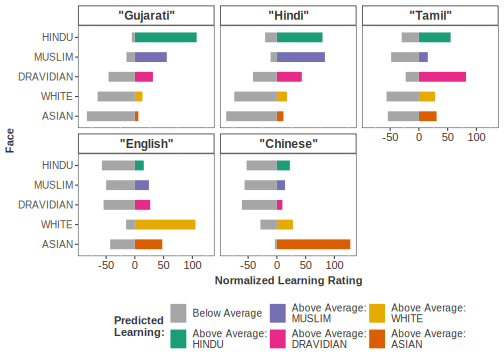
\includegraphics[width=\linewidth]{figures/std_plots/learning_diverging_barplot_colored.png}
    \caption{Normalized Learning Predictions for Each Face, by Language. Diverging bars reflect the number of children predicting below- versus above-average learning for each face, normalized by language. Panels display data for each language; below-average (negative) counts appear in grey, while above-average counts are colored by face.
    \label{fig:faces-learning-diverging}}
\vspace{-7pt}
\end{figure}
\subsection*{Linguistic Essentialism} 
Finally, we explored children's tendency to essentialize language via their intuitions of how well each of five languages (Gujarati, Hindi, Tamil, English, and Chinese) would be learned by each speaker, under identical learning conditions. 
We fit linear models to children's learning ratings (1--3) for each face individually, with language and child age at minimum as predictors, and the interaction between language and child age when its inclusion improved model fit (see Figure~\ref{fig:faces-learning-score} and Table~\learningmeanstab\ for mean estimated learning success for each face, by child grade).
\paragraph*{North Indian Hindu face {\small{(HINDU)}}} 
There was a significant effect of language ($F(4, 547)=59$, $p<.001$), such that children tended to predict greater learning of Gujarati ($b=2.73$ [$2.63, 2.85]$) by the \textsc{hindu} face, and reliably worse learning of Chinese ($b=-1.08$ [$-1.25, -0.92]$), English ($b=-0.77$ [$-0.94, -0.62]$), and Tamil ($b=-0.66$ [$-0.83, -0.50]$).

\paragraph*{Muslim face {\small{(MUSLIM)}}} 
There was a significant effect of language ($F(4, 499)=70.54$, $p<.001$), such that children tended to predict greater learning of Gujarati ($b=2.34$ [$2.22, 2.45]$) and Hindi ($b=0.38$ [$0.22, 0.54]$) by the \textsc{muslim} face, and lesser learning of Chinese ($b=-0.81$ [$-0.98, -0.65]$), English ($b=-0.30$ [$-0.46, -0.14]$), and Tamil ($b=-0.71$ [$-0.88, -0.56]$). 
With age, children also predicted greater learning for the \textsc{muslim} face slightly more often ($b=0.04$ [$0.00, 0.08]$; $F(1, 499)=4.56$, $p<.05$).

\paragraph*{South Indian Hindu face {\small{(DRAVIDIAN)}}} 
There was a significant effect of language ($F(4, 487)=21.72$, $p<.001$), such that children tended to predict greater learning by the \textsc{dravidian} face for Gujarati ($b=1.93$ [$1.79, 2.08]$), Tamil ($b=0.41$ [$0.21, 0.61]$), and Hindi ($b=0.30$ [$0.10, 0.50]$), and lesser learning for Chinese ($b=-0.47$ [$-0.68, -0.27]$).

\paragraph*{White face {\small{(WHITE)}}} 
There were significant effects of language ($F(4, 539)=63.21$, $p<.001$), child age ($F(4, 539)=6.15$, $p<.01$), and their interaction ($F(1, 539)=10.57$, $p<.01$), such that children tended to predict greater learning by the \textsc{white} face for Gujarati ($b=1.67$ [$1.56, 1.79]$), English ($b=1.10$ [$0.93, 1.26]$), Chinese ($b=0.20$ [$0.03, 0.37]$), and Hindi ($b=0.17$ [$0.00, 0.33]$), to different degrees with age. 
As children got older, their learning predictions for Gujarati attenuated ($b=-0.13$ [$-0.26, -0.04]$), while their expectations for English ($b=0.20$ [$0.10, 0.31]$) and Chinese ($b=0.15$ [$0.04, 0.26]$) further increased. 
%significant effects of language, child age, and their interaction: more essentialist with age 
\paragraph*{East Asian face {\small{(ASIAN)}}}
There was a significant effect of language ($F(4, 486)=80.32$, $p<.001$) and interaction between language and child age ($F(4, 486)=3.84$, $p<.01$): children projected greater learning by the \textsc{asian} face for Gujarati ($b=1.43$ [$1.29, 1.56]$), Chinese ($b=1.40$ [$1.21, 1.60]$), English ($b=1.40$ [$0.61, 0.99]$), Hindi ($b=0.22$ [$0.03, 0.40]$), and Tamil ($b=0.33$ [$0.14, 0.52]$). 

In sum, children predicted that individuals of some ethnicities and religions would be better at learning particular languages, and these predictions often grew stronger with age (see Figures~\ref{fig:faces-learning-score} and \ref{fig:faces-learning-diverging}). 
%children's predictions of different individuals' language-learning capacity differed by thi ethnic/religious identities, and often showed greater divergence across faces with age.
\begin{figure}[h]
    \centering
    \includegraphics[width=\linewidth]{figures/std_plots/id_accuracy_std.png}
    \caption{Language Identification Accuracy by Grade. Points plot mean accuracy by grade, with error bars representing 95\% bootstrapped confidence intervals. Each line represents a different language.}
    \label{fig:lang-id-by-std}
\vspace{-7pt}
\end{figure}
\subsection*{Language Identification}
Mean accuracy by language and grade are plotted in Figure~\ref{fig:faces-learning-score}. Children became more accurate at identifying the audio clips with age (e.g., 50\% overall accuracy in $3^{\textnormal{rd}}$ grade and 68\% accuracy in $7^{\textnormal{th}}$ grade). Children struggled most with identifying Urdu ($M=0.11$ [$0.05, 0.17]$), Tamil ($M=0.33$ [$0.25, 0.41]$), and Marathi ($M=0.59$ [$0.51, 0.68]$). 
Interestingly, children showed preferential associations with languages---the same ones that would become the most common associations in $7^{\textnormal{th}}$ grade---even when they could not actually identify the language. For example, $3^{\textnormal{rd}}$-graders who were unable to name Urdu still selected the \textsc{muslim} face as the speaker for the Urdu audio clips and `Muslim' as the speaker's religion on 45\% of trials, and Gujarat as the speaker's geographic origin on 70\% of trials. Similarly, $3^{\textnormal{rd}}$-graders who failed to identify ``Chinese'' still selected the \textsc{asian} face for the Mandarin audio clips on 46\% of trials, and identified the Mandarin speaker as ``foreign'' on 25\% of trials. And $3^{\textnormal{rd}}$-graders who were unable to name Tamil or Marathi nonetheless recognized their speakers as likely ``from another place in India'' (48\% of trials by children who couldn't identify Tamil, and 31\% of trials by children who couldn't identify Marathi).  %45% Urdu-muslim, 15\% Marathi-Hindu
% Marathi-hindu face 24%  (only in those who got Marathi id wrong)
% Tamil-dravidian 12%
% Tamil-different state 48%
% Marathi-different state 31%
\section*{General Discussion}
Despite the prevalence of multilingualism globally, most research on sociolinguistic development has focused on monolingual children in environments with relatively little linguistic diversity, and, as such, has not systematically addressed what children take different languages to socially signify. The present study aimed to fill this gap by tracing the development of social inferences and essentialist beliefs about languages among multilingual children and adolescents in Gujarat, India. Although multilingual experience could in principle make children less likely to make stereotyping inferences about speakers of a language---since multilingual children might expect an individual to know multiple languages beyond the one they are currently using---we were interested in whether children in our sample might nevertheless exhibit social associations with languages across a variety of dimensions. To examine this possibility, we presented children with audio clips of eight different languages or dialects (unlabeled by language names) and probed associations with speakers' geographic origin, religion, wealth, and facial appearance (while also probing the latter using only language names). We also measured essentialist beliefs about language by asking children whether individuals of different ethnic/religious identities would vary in their ability to learn the different languages.

Children in our sample selectively linked the different languages we presented with the different social dimensions we probed, and these patterns generally became more reliable with age. Specifically, with respect to geographical origin, with age, children progressively identified speakers of audio clips of Gujarati as being from Gujarat while judging speakers of the Marathi, Hindi, Urdu and Tamil clips as originating from another state of India and judging speakers of the U.S. English, Mandarin and Indian English clips as originating from outside of India. With respect to religion, with age, children progressively assumed that speakers of the Gujarati clips were Hindu, that speakers of the Urdu clips were Muslim, and that speakers of the U.S. and Indian English clips were Christian. With respect to wealth, children progressively inferred that speakers of the Gujarati, Mandarin, U.S. and Indian English clips had more money than they did. Finally, with age, children also selectively linked languages with faces that stereotypically corresponded to different ethnic or religious identities, for example pairing speakers of Gujarati with North Indian faces, Urdu with Muslim faces, Mandarin with East Asian faces, and American and Indian English with white faces; interestingly, these tendencies were even more pronounced when facial associations were probed with language names (e.g., ``Who is speaking English?''), and children also appeared to understand these associations between language and ethnic/religious identity in an essentialist manner (e.g., judging that a white person would be better able to learn English than individuals of other ethnic groups, even when told that none of these individuals had any prior experience with English). 

Perhaps because most prior work in sociolinguistic development has been conducted with monolingual children with relatively little multilingual experience, these studies have typically assessed children's social associations with a small number of varieties of the same language (e.g., \cite{weatherhead2019preschoolers}; \cite{mccullough2019regional}; \cite{kinzler2013northern}) or have contrasted associations involving children's own language with those involving a single, unfamiliar language (e.g.,  \cite{liberman2017preverbal}; \cite{hirschfeld1997young}; \cite{kinzler2012children}; \cite{kinzler2007native}; \cite{moon1993two}). Our findings extend this prior work in suggesting that---when faced with significantly greater linguistic and social variability---children can nevertheless attribute social features to languages in systematic and nuanced ways. Notably, the sociolinguistic associations that children in our sample exhibited could not be explained by a simple tendency to judge that people who spoke different languages than they did would be different from them, in general (\cite{hirschfeld1997young}), as such a heuristic would have predicted that our participants would have made largely similar judgments about multiple languages that we probed that they did not themselves speak (e.g., making similar judgments about Tamil, Urdu, Marathi and Mandarin, which were unfamiliar to many of our participants), which they generally did not do.\footnote{One example of a case in which children may have used a ``different language = different than me'' strategy was in their judgments of the religion of Tamil speakers. With age, children were more likely to identify Tamil speakers as Buddhist, an association that is unconnected to actual fact. Tamil was unfamiliar to many of our participants, and lacking any evidence about the religion of speakers of these languages, children may have guessed that they practiced a religion (Buddhism) that was unfamiliar to them.} 
Relatedly, children's responses could not be explained by a general tendency to project positive traits onto individuals who spoke the same languages they did (e.g., judging those speakers as nicer or smarter; \cite{santhanagopalan2021nationality}), given that some of the dimensions that we probed---including facial appearance, geographic origin, and religion---are not easily organized along a positive--negative continuum.

Instead, children in our sample developed specific sociolinguistic associations, which often reflected regularities in the real world: e.g., Tamil and Marathi \textit{are} languages that derive from other regions of India (outside of Gujarat), Urdu speakers \textit{do} tend to be Muslim, Tamil speakers \textit{do} tend to look Dravidian, and U.S. English speakers \textit{do} tend to have more wealth than many people who live in Gujarat, due to global wealth inequalities. (One striking exception to this pattern of providing veridical associations were children's judgments of speakers of Indian English, which we return to below). 

Our findings provide preliminary evidence that children in our sample may have constructed these and other associations both by attending to ``bottom-up'' correlations in their real-world environmental experience (e.g., hearing a language spoken and attending to characteristics of the speakers), but also via ``top-down'' transmission of information about speakers of different languages (e.g., messages about a language and its community of speakers). Attesting to the role of bottom-up experience, even children who could not identify the languages of audio clips nevertheless exhibited systematic associations with those clips (e.g., linking Mandarin clips with East Asian faces). And speaking to the role of higher-level conceptual knowledge, recall that children were more systematic in linking different languages with stereotypical faces when these associations were probed via language name (e.g., ``Who is speaking Urdu?''), compared to when they were probed with unlabeled audio clips alone. This latter pattern of findings suggests that children's associations between languages and ethnic/religious identity were partly linked to higher-level conceptual knowledge about those languages (e.g., that speakers of ``Urdu'' tend to be Muslim), such that this knowledge could be cued by language names without necessarily being accessible from listening to audio clips alone (e.g., for children who did not recognize an audio clip as containing ``Urdu''). It will be important to explore the interplay of bottom-up and top-down processes in the development of sociolinguistic associations in future work.

Based on the intuition that a multilingual child in a multilingual context might assume that other people will know multiple languages, our findings present a puzzle: Why were children in our sample so willing to make social inferences about a speaker based on the language they were using when they could easily have assumed that the speaker knew other languages, as well? One intriguing possibility is that children's responses did not reflect their beliefs about actual real-world speakers, \textit{per se}, but instead reflected their understanding of the different, idealized \textit{personae} that a speaker can embody and project when they use different languages. Sociolinguistic theory defines \textit{personae} as ``\ldots holistic, ideological social types that are recognizably linked with ways of being and speaking'' (\cite{donofrio2020personae},  p. 1; see also \cite{d2016social}), and has used this construct to characterize the social identities associated with styles within a language that speakers draw upon: e.g., an English speaker can perform shallowness by using features of the ``Valley Girl'' style (e.g., including uptalk and using `like' as a discourse marker; \cite{pratt2017jaw}; \cite{d2015persona}). We suggest that this construct can be fruitfully extended to characterize how people make sense of the social meaning of different languages within multilingual contexts: e.g., such that, for children in our sample, the use of Gujarati evokes a local, Hindu, and North Indian persona, the use of English evokes a foreign, wealthy, white, and Christian persona, and so on. 

This proposal may help make sense of a striking pattern of findings we observed when probing children's judgments of speakers of Indian English audio clips. Children generally judged these speakers similarly to speakers of American English clips---as white, originating from outside of India, and Christian. Moreover, these surprising tendencies often became more---rather than less---pronounced with age.\footnote{The exception to this generalization is children's attributions of greater relative wealth to the speakers of Indian English, which did not become particularly more pronounced with age.} 
These findings are unexpected if we take children's responses to reflect their beliefs about the actual characteristics of speakers in their real-world environment, given that our participants were students at an English-medium school who heard ample Indian English spoken by teachers, staff, and peers from their community---who were themselves rarely Christian and never white. Instead, we suggest that, for children in our sample, the use of Indian English evokes an idealized persona that is foreign, Christian, and white, which may itself be shaped by beliefs about and associations with speakers of British and American English. %(for which these associations have more basis in fact). 
Understanding the role of personae in children's developing sociolinguistic competence will be an important direction for future work.

A final striking finding that emerged from our study was that children exhibited essentialist beliefs about language learning---e.g., judging that, compared to individuals of other ethnicities, and even if they had no prior experience with the language, a white person would be better able to learn English, a North Indian person would be better able to learn Hindi and Gujarati, an East Asian person would be better able to learn Chinese, and so on. Such responses typically became more pronounced with age, which stands in contrast to prior work suggesting that essentialism of language decreases after the preschool years (\cite{kinzler2012children}) and is diminished among bilingual children (\cite{byers2015bilingualism}; \cite{dautel2018once}). Yet it is important to note that these prior studies employed different measures of essentialism than we did here, asking whether children view language as biologically- or culturally-transmitted (e.g., via switched-at-birth paradigms; \cite{hirschfeld1997young}; \cite{byers2015bilingualism}), or by evaluating the stability of language relative to race over the lifespan (e.g., by asking whether a child who was white and spoke English would be more likely to change their language or race as an adult; \cite{kinzler2012children}; \cite{dautel2018once}). It is possible that language learning ability is particularly likely to be essentialized, especially for individuals who experience the difficulty of trying to learn a new language later in life (as was the case for many of our participants, who were non-native learners of English), since this difficulty could lead individuals to assume that those who speak other languages fluently possess an innate, biological advantage for those languages. It will be interesting in future work to explore how different facets of linguistic essentialism emerge and change across the lifespan, and how this might be shaped by multilingual experience.

%\textbf{Conclusion}
%This work represents an important step towards understanding the origins and import of children's associations between languages and the social world. By sampling across middle childhood and early adolescence, in a context where children can assume speakers are multilingual
%even when can assume speakers speak multiple languages, ind langs still meaningful, shedding light on how to interpret assumptions as about speakers 

%how language users' inferences from a speaker's language develop, by sampling them across middle childhood to early adolescence, in a context where ...sophisticated inferences on the basis of the language someone speaks develop in a 
%This work represents an important step towards understanding how sociolinguistic development is influenced by experience in a multilingual environment. Even though anyone can learn any language provided they are exposed to that language early in life, language knowledge is not randomly distributed across people; instead, similar people tend to speak the same language. This allows listeners to make rich inferences based on the language or dialect a person speaks. As discussed, it is well established that in monolingual contexts, even infants use language as a cue to social categorization. It is plausible that this phenomenon might not extend to multilingual environments, but, here, we have shown that children in multilingual environment also derive complex social inferences based on language. These inferences are influenced both by culturally acquired knowledge and direct experience. This evidence raises an intriguing question: how do children navigate and create their own sociolinguistic identities within this diverse linguistic landscape? In a setting where speakers are proficient in multiple languages, each individual must make choices about the appropriate language to speak in specific situations (e.g., with family or friends, at school, at work, in the street, etc.). The strong associations that children learn between languages and attributed such as wealth or physical appearance further complicate these decisions. The act of choosing which language to speak becomes a nuanced process of constructing a sociolinguistic persona, and it raises the fascinating question of how children decide to shape this persona. Overall, the research presented here opens a window into the complex interplay of language and social cognition in multilingual environments and invites further exploration into how children perceive and navigate their complex social landscapes. 

\printbibliography
\clearpage
\begin{appendix}
\begin{table}[t]
%\vspace{-50pt}
 \centering
\caption{Mean Geographic Origin Association by Speaker Language and Child Grade}
\begin{footnotesize}
\renewcommand{\tabcolsep}{0.15cm}
\label{tab:geographic-origins-means}
\begin{tabular}{p{.1in}lrrrrrrrrr}
\toprule
 &  & \multicolumn{3}{c}{\textbf{3rd}} & \multicolumn{3}{c}{\textbf{5th}} & \multicolumn{3}{c}{\textbf{7th}} \\
\cline{3-5} \cline{6-8} \cline{9-11}\\[-.75em]
&  & \textit{n} & \textit{M} & [95\% \textit{CI}] &  \textit{n} & \textit{M} & [95\% \textit{CI}] &  \textit{n}  & \textit{M} & [95\% \textit{CI}]\\
\midrule
\multicolumn{11}{l}{\textbf{Gujarat (Same State as Me)}}\\
 & Gujarati & 17 & 0.44 & [0.28, 0.60] & 72 & 0.74 & [0.65, 0.82] & 72 & 0.77 & [0.69, 0.85]\\

 & Hindi & 31 & 0.79 & [0.66, 0.92] & 48 & 0.49 & [0.40, 0.59] & 63 & 0.68 & [0.59, 0.77]\\

 & Urdu & 26 & 0.68 & [0.53, 0.84] & 49 & 0.51 & [0.40, 0.61] & 55 & 0.59 & [0.48, 0.68]\\

 & Marathi & 16 & 0.41 & [0.26, 0.56] & 28 & 0.29 & [0.20, 0.38] & 31 & 0.33 & [0.25, 0.43]\\

 & Tamil & 12 & 0.31 & [0.17, 0.45] & 15 & 0.15 & [0.08, 0.24] & 6 & 0.06 & [0.02, 0.12]\\

 & English (India) & 12 & 0.32 & [0.17, 0.47] & 10 & 0.10 & [0.04, 0.17] & 10 & 0.11 & [0.05, 0.17]\\

 & English (U.S.) & 11 & 0.28 & [0.15, 0.43] & 5 & 0.05 & [0.01, 0.1] & 8 & 0.08 & [0.03, 0.15]\\

& Mandarin & 4 & 0.10 & [0.02, 0.21] & 4 & 0.04 & [0.01, 0.08] & 1 & 0.01 & [0.00, 0.03]\\

\midrule
\multicolumn{11}{l}{\textbf{India (Different State)}}\\
  & Gujarati & 8 & 0.21 & [0.08, 0.35] & 16 & 0.16 & [0.10, 0.24] & 14 & 0.15 & [0.09, 0.23]\\

 & Hindi & 3 & 0.08 & [0.00, 0.17] & 46 & 0.47 & [0.38, 0.57] & 29 & 0.31 & [0.22, 0.41]\\

 & Urdu & 8 & 0.21 & [0.10, 0.34] & 42 & 0.43 & [0.33, 0.54] & 33 & 0.35 & [0.26, 0.46]\\

 & Marathi & 13 & 0.33 & [0.19, 0.49] & 54 & 0.56 & [0.46, 0.65] & 56 & 0.60 & [0.50, 0.71]\\

 & Tamil & 17 & 0.44 & [0.29, 0.59] & 51 & 0.53 & [0.43, 0.63] & 67 & 0.71 & [0.62, 0.80]\\

 & English (India) & 6 & 0.16 & [0.05, 0.28] & 18 & 0.19 & [0.11, 0.27] & 19 & 0.20 & [0.13, 0.29]\\

 & English (U.S.) & 11 & 0.28 & [0.14, 0.43] & 25 & 0.26 & [0.18, 0.35] & 14 & 0.15 & [0.08, 0.22]\\

& Mandarin & 7 & 0.18 & [0.07, 0.32] & 19 & 0.20 & [0.12, 0.28] & 19 & 0.20 & [0.13, 0.28]\\

\midrule
\multicolumn{11}{l}{\textbf{Foreign (Outside India)}}\\
& Gujarati & 13 & 0.33 & [0.19, 0.49] & 9 & 0.09 & [0.04, 0.15] & 7 & 0.08 & [0.02, 0.13]\\

 & Hindi & 5 & 0.13 & [0.03, 0.24] & 2 & 0.02 & [0.00, 0.05] & 0 & --- & ---\\

 & Urdu & 3 & 0.08 & [0.00, 0.18] & 4 & 0.04 & [0.01, 0.08] & 4 & 0.04 & [0.01, 0.09]\\

 & Marathi & 9 & 0.23 & [0.10, 0.38] & 14 & 0.14 & [0.08, 0.22] & 4 & 0.04 & [0.01, 0.09]\\

 & Tamil & 10 & 0.26 & [0.12, 0.38] & 30 & 0.31 & [0.21, 0.40] & 14 & 0.15 & [0.09, 0.22]\\

 & English (India) & 18 & 0.47 & [0.32, 0.63] & 68 & 0.71 & [0.61, 0.80] & 63 & 0.67 & [0.59, 0.77]\\

 & English (U.S.) & 16 & 0.41 & [0.27, 0.56] & 65 & 0.67 & [0.58, 0.77] & 70 & 0.74 & [0.64, 0.82]\\

& Mandarin & 25 & 0.64 & [0.47, 0.79] & 71 & 0.73 & [0.64, 0.82] & 70 & 0.75 & [0.67, 0.83]\\

\midrule
\multicolumn{11}{l}{\textbf{No Opinion}}\\
& Gujarati & 1 & 0.03 & [0.00, 0.08] & 0 & --- & --- & 0 & --- & ---\\

 & Hindi & 0 & --- & --- & 1 & 0.01 & [0.00, 0.03] & 1 & 0.01 & [0.00, 0.03]\\

 & Urdu & 1 & 0.03 & [0.00, 0.09] & 2 & 0.02 & [0.00, 0.05] & 2 & 0.02 & [0.00, 0.05]\\

 & Marathi & 1 & 0.03 & [0.00, 0.08] & 1 & 0.01 & [0.00, 0.03] & 2 & 0.02 & [0.00, 0.05]\\

 & Tamil & 0 & --- & --- & 1 & 0.01 & [0.00, 0.03] & 7 & 0.07 & [0.03, 0.13]\\

 & English (India) & 2 & 0.05 & [0.00, 0.14] & 0 & --- & --- & 2 & 0.02 & [0.00, 0.05]\\

 & English (U.S.) & 1 & 0.03 & [0.00, 0.08] & 2 & 0.02 & [0.00, 0.05] & 3 & 0.03 & [0.00, 0.07]\\

& Mandarin & 3 & 0.08 & [0.00, 0.17] & 3 & 0.03 & [0.00, 0.07] & 3 & 0.03 & [0.00, 0.08]\\
\bottomrule
\end{tabular}
\end{footnotesize}
\end{table}

\clearpage
\thispagestyle{empty}
\begin{table}[t]
\vspace{-20pt}
\centering
\caption{Mean Religious Association by Speaker Language and Child Grade\label{tab:religion-means}}\\
\begin{footnotesize}
%\renewcommand{\tabcolsep}{0.15cm}
\begin{tabular}{p{.1in}lrrrrrrrrr}
%\begin{tabular}{p{.1in}lrrrrrrrrr}
\toprule
 &  & \multicolumn{3}{c}{\textbf{3rd}} & \multicolumn{3}{c}{\textbf{5th}} & \multicolumn{3}{c}{\textbf{7th}} \\
\cline{3-5} \cline{6-8} \cline{9-11}\\[-.75em]
&  & \textit{n} & \textit{M} & [95\% \textit{CI}] &  \textit{n} & \textit{M} & [95\% \textit{CI}] &  \textit{n}  & \textit{M} & [95\% \textit{CI}]\\
\midrule
\multicolumn{11}{l}{\textbf{Hindu}}\\
 & Gujarati & 12 & 0.32 & [0.18, 0.49] & 72 & 0.71 & [0.61, 0.79] & 67 & 0.71 & [0.62, 0.80]\\

 & Hindi & 11 & 0.29 & [0.14, 0.43] & 54 & 0.53 & [0.45, 0.63] & 50 & 0.53 & [0.44, 0.63]\\

 & Urdu & 12 & 0.33 & [0.19, 0.48] & 46 & 0.46 & [0.36, 0.55] & 44 & 0.47 & [0.38, 0.57]\\

 & Marathi & 7 & 0.18 & [0.07, 0.32] & 48 & 0.48 & [0.38, 0.57] & 56 & 0.60 & [0.50, 0.69]\\

 & Tamil & 9 & 0.24 & [0.12, 0.38] & 17 & 0.17 & [0.10, 0.25] & 10 & 0.11 & [0.05, 0.17]\\

 & English (India) & 10 & 0.27 & [0.14, 0.42] & 15 & 0.15 & [0.08, 0.23] & 9 & 0.10 & [0.04, 0.16]\\

 & English (U.S.) & 8 & 0.21 & [0.08, 0.35] & 5 & 0.05 & [0.01, 0.09] & 7 & 0.07 & [0.02, 0.13]\\

& Mandarin & 4 & 0.11 & [0.02, 0.21] & 3 & 0.03 & [0.00, 0.07] & 0 & --- & ---\\

\midrule
\multicolumn{11}{l}{\textbf{Muslim}}\\
 & Gujarati & 10 & 0.27 & [0.14, 0.41] & 7 & 0.07 & [0.03, 0.12] & 11 & 0.12 & [0.05, 0.18]\\

 & Hindi & 19 & 0.50 & [0.33, 0.66] & 34 & 0.34 & [0.25, 0.43] & 26 & 0.28 & [0.19, 0.36]\\

 & Urdu & 21 & 0.58 & [0.42, 0.74] & 40 & 0.40 & 0.30, 0.49] & 39 & 0.42 & [0.32, 0.53]\\

 & Marathi & 9 & 0.24 & [0.11, 0.37] & 10 & 0.10 & [0.05, 0.16] & 1 & 0.01 & [0.00, 0.03]\\

 & Tamil & 9 & 0.24 & [0.10, 0.37] & 11 & 0.11 & [0.05, 0.18] & 6 & 0.06 & [0.02, 0.12]\\

 & English (India) & 5 & 0.14 & [0.03, 0.26] & 12 & 0.12 & [0.06, 0.19] & 1 & 0.01 & [0.00, 0.03]\\

 & English (U.S.) & 4 & 0.11 & [0.03, 0.21] & 13 & 0.13 & [0.07, 0.20] & 3 & 0.03 & [0.00, 0.07]\\
 & Mandarin & 4 & 0.11 & [0.02, 0.21] & 9 & 0.09 & [0.04, 0.15] & 6 & 0.06 & [0.02, 0.12]\\
 \midrule
\multicolumn{11}{l}{\textbf{Jain}}\\
  & Gujarati & 7 & 0.19 & [0.08, 0.32] & 10 & 0.10 & [0.05, 0.16] & 3 & 0.03 & [0.00, 0.06]\\

 & Hindi & 4 & 0.11 & [0.02, 0.21] & 8 & 0.08 & [0.03, 0.14] & 9 & 0.10 & [0.04, 0.15]\\

 & Urdu & 0 & --- & --- & 10 & 0.10 & [0.04, 0.16] & 3 & 0.03 & [0.00, 0.07]\\

 & Marathi & 8 & 0.21 & [0.09, 0.34] & 16 & 0.16 & [0.09, 0.23] & 5 & 0.05 & [0.02, 0.11]\\

 & Tamil & 7 & 0.18 & [0.06, 0.31] & 30 & 0.30 & [0.22, 0.39] & 18 & 0.19 & [0.12, 0.27]\\

 & English (India) & 6 & 0.16 & [0.05, 0.30] & 16 & 0.16 & [0.10, 0.23] & 6 & 0.07 & [0.02, 0.12]\\

 & English (U.S.) & 5 & 0.13 & [0.03, 0.24] & 20 & 0.20 & [0.12, 0.28] & 5 & 0.05 & [0.01, 0.09]\\

& Mandarin & 7 & 0.18 & [0.07, 0.31] & 18 & 0.18 & [0.11, 0.26] & 12 & 0.13 & [0.07, 0.20]\\
 \midrule
\multicolumn{11}{l}{\textbf{Christian}}\\
 & Gujarati & 5 & 0.14 & [0.03, 0.26] & 4 & 0.04 & [0.01, 0.08] & 3 & 0.03 & [0.00, 0.07]\\

 & Hindi & 0 & --- & --- & 4 & 0.04 & [0.01, 0.08] & 1 & 0.01 & [0.00, 0.03]\\

 & Urdu & 4 & 0.11 & [0.02, 0.22] & 3 & 0.03 & [0.00, 0.07] & 0 & --- & ---\\

 & Marathi & 6 & 0.16 & [0.05, 0.28] & 8 & 0.08 & [0.03, 0.14] & 4 & 0.04 & [0.01, 0.09]\\

 & Tamil & 8 & 0.21 & [0.08, 0.35] & 16 & 0.16 & [0.09, 0.24] & 5 & 0.05 & [0.01, 0.11]\\

 & English (India) & 12 & 0.32 & [0.18, 0.48] & 32 & 0.32 & [0.24, 0.41] & 48 & 0.52 & [0.42, 0.62]\\

 & English (U.S.) & 14 & 0.37 & [0.22, 0.52] & 36 & 0.36 & [0.27, 0.46] & 40 & 0.42 & [0.33, 0.52]\\
& Mandarin & 10 & 0.26 & [0.14, 0.41] & 20 & 0.20 & [0.13, 0.28] & 21 & 0.23 & [0.15, 0.31]\\
 \midrule
\multicolumn{11}{l}{\textbf{Buddhist}}\\
& Gujarati & 3 & 0.08 & [0.00, 0.18] & 4 & 0.04 & [0.01, 0.08] & 3 & 0.03 & [0.00, 0.07]\\

 & Hindi & 3 & 0.08 & [0.00, 0.18] & 0 & --- & --- & 2 & 0.02 & [0.00, 0.05]\\

 & Urdu & 0 & --- & --- & 1 & 0.01 & [0.00, 0.03] & 3 & 0.03 & [0.00, 0.07]\\

 & Marathi & 5 & 0.13 & [0.05, 0.25] & 10 & 0.10 & [0.05, 0.16] & 14 & 0.15 & [0.07, 0.22]\\

 & Tamil & 2 & 0.05 & [0.00, 0.13] & 18 & 0.18 & [0.11, 0.25] & 31 & 0.33 & [0.23, 0.43]\\

 & English (India) & 1 & 0.03 & [0.00, 0.09] & 7 & 0.07 & [0.03, 0.13] & 4 & 0.04 & [0.01, 0.09]\\

 & English (U.S.) & 4 & 0.11 & [0.02, 0.21] & 10 & 0.10 & [0.05, 0.16] & 8 & 0.08 & [0.03, 0.15]\\

& Mandarin & 5 & 0.13 & [0.03, 0.24] & 16 & 0.16 & [0.09, 0.23] & 9 & 0.10 & [0.04, 0.16]\\
 \midrule
\multicolumn{11}{l}{\textbf{No Opinion}}\\
& Gujarati & 0 & --- & --- & 4 & 0.04 & [0.01, 0.08] & 7 & 0.07 & [0.02, 0.14]\\

 & Hindi & 1 & 0.03 & [0.00, 0.08] & 1 & 0.01 & [0.00, 0.03] & 6 & 0.06 & [0.02, 0.12]\\

 & Urdu & 0 & --- & --- & 1 & 0.01 & [0.00, 0.03] & 5 & 0.05 & [0.01, 0.11]\\

 & Marathi & 3 & 0.08 & [0.00, 0.17] & 9 & 0.09 & [0.04, 0.15] & 14 & 0.15 & [0.07, 0.22]\\

 & Tamil & 3 & 0.08 & [0.00, 0.18] & 9 & 0.09 & [0.04, 0.15] & 25 & 0.27 & [0.18, 0.35]\\

 & English (India) & 3 & 0.08 & [0.00, 0.18] & 18 & 0.18 & [0.11, 0.26] & 24 & 0.26 & [0.18, 0.35]\\

 & English (U.S.) & 3 & 0.08 & [0.00, 0.17] & 17 & 0.17 & [0.10, 0.24] & 32 & 0.34 & [0.24, 0.43]\\

& Mandarin & 8 & 0.21 & [0.09, 0.35] & 35 & 0.35 & [0.25, 0.45] & 45 & 0.48 & [0.38, 0.59]\\

\bottomrule
%\end{tabular}
\end{tabular}
\end{footnotesize}
\end{table}
\clearpage
\begin{table}[t]
\centering
\caption{Mean Wealth Association by Speaker Language and Child Grade}
\begin{footnotesize}
\label{tab:wealth-means}
\begin{tabular}{p{.1in}lrrrrrrrrr}
\toprule
 &  & \multicolumn{3}{c}{3rd} & \multicolumn{3}{c}{5th} & \multicolumn{3}{c}{7th} \\
\cline{3-5} \cline{6-8} \cline{9-11}
&  & \textit{n} & \textit{M} & [95\% \textit{CI}] &  \textit{n} & \textit{M} & [95\% \textit{CI}] &  \textit{n}  & \textit{M} & [95\% \textit{CI}]\\
\midrule
\multicolumn{11}{l}{\textbf{Less Money}}\\
 & Gujarati & 5 & 0.13 & [0.03, 0.25] & 24 & 0.24 & [0.16, 0.32] & 12 & 0.13 & [0.07, 0.2]\\

 & Hindi & 9 & 0.24 & [0.12, 0.39] & 22 & 0.22 & [0.14, 0.31] & 12 & 0.13 & [0.06, 0.2]\\

 & Urdu & 7 & 0.18 & [0.07, 0.31] & 16 & 0.16 & [0.09, 0.23] & 8 & 0.09 & [0.03, 0.15]\\

 & Marathi & 6 & 0.17 & [0.05, 0.3] & 23 & 0.23 & [0.15, 0.31] & 8 & 0.09 & [0.03, 0.15]\\

 & Tamil & 6 & 0.16 & [0.05, 0.29] & 25 & 0.25 & [0.17, 0.33] & 18 & 0.19 & [0.12, 0.28]\\

 & English (India) & 8 & 0.22 & [0.09, 0.35] & 13 & 0.13 & [0.07, 0.2] & 10 & 0.11 & [0.05, 0.18]\\

 & English (U.S.) & 5 & 0.13 & [0.05, 0.24] & 9 & 0.09 & [0.04, 0.15] & 6 & 0.06 & [0.02, 0.12]\\

& Mandarin & 4 & 0.11 & [0.02, 0.21] & 8 & 0.08 & [0.03, 0.13] & 12 & 0.13 & [0.06, 0.19]\\
\midrule
\multicolumn{11}{l}{\textbf{As Much Money}}\\
 & Gujarati & 13 & 0.34 & [0.2, 0.5] & 43 & 0.43 & [0.33, 0.52] & 55 & 0.59 & [0.5, 0.69]\\

 & Hindi & 13 & 0.35 & [0.2, 0.51] & 40 & 0.40 & [0.31, 0.5] & 54 & 0.57 & [0.47, 0.67]\\

 & Urdu & 19 & 0.49 & [0.33, 0.64] & 49 & 0.49 & [0.39, 0.58] & 55 & 0.59 & [0.49, 0.68]\\

 & Marathi & 14 & 0.39 & [0.23, 0.56] & 38 & 0.38 & [0.28, 0.47] & 41 & 0.44 & [0.34, 0.53]\\

 & Tamil & 15 & 0.39 & [0.25, 0.56] & 40 & 0.40 & [0.31, 0.49] & 37 & 0.40 & [0.3, 0.51]\\

 & English (India) & 14 & 0.38 & [0.24, 0.54] & 22 & 0.22 & [0.14, 0.3] & 29 & 0.31 & [0.22, 0.39]\\

 & English (U.S.) & 11 & 0.29 & [0.15, 0.45] & 32 & 0.32 & [0.23, 0.41] & 38 & 0.40 & [0.31, 0.51]\\

& Mandarin & 7 & 0.19 & [0.07, 0.32] & 25 & 0.25 & [0.16, 0.33] & 19 & 0.20 & [0.13, 0.3]\\
\midrule
\multicolumn{11}{l}{\textbf{More Money}}\\
 & Gujarati & 15 & 0.39 & [0.25, 0.55] & 29 & 0.29 & [0.2, 0.39] & 11 & 0.12 & [0.06, 0.18]\\

 & Hindi & 12 & 0.32 & [0.17, 0.48] & 31 & 0.31 & [0.22, 0.4] & 11 & 0.12 & [0.05, 0.18]\\

 & Urdu & 12 & 0.31 & [0.17, 0.46] & 34 & 0.34 & [0.24, 0.43] & 12 & 0.13 & [0.06, 0.19]\\

 & Marathi & 12 & 0.33 & [0.18, 0.5] & 33 & 0.33 & [0.24, 0.42] & 11 & 0.12 & [0.05, 0.18]\\

 & Tamil & 14 & 0.37 & [0.21, 0.53] & 30 & 0.30 & [0.21, 0.38] & 6 & 0.06 & [0.02, 0.12]\\

 & English (India) & 13 & 0.35 & [0.19, 0.5] & 61 & 0.62 & [0.52, 0.71] & 32 & 0.34 & [0.24, 0.44]\\

 & English (U.S.) & 21 & 0.55 & [0.4, 0.71] & 56 & 0.55 & [0.46, 0.66] & 25 & 0.27 & [0.18, 0.37]\\

 & Mandarin & 19 & 0.51 & [0.37, 0.67] & 57 & 0.56 & [0.46, 0.67] & 32 & 0.34 & [0.26, 0.45]\\
\midrule
\multicolumn{11}{l}{\textbf{No Opinion}}\\
 & Gujarati & 5 & 0.13 & [0.03, 0.25] & 5 & 0.05 & [0.01, 0.09] & 15 & 0.16 & [0.09, 0.24]\\

 & Hindi & 3 & 0.08 & [0, 0.17] & 7 & 0.07 & [0.02, 0.13] & 17 & 0.18 & [0.11, 0.26]\\

 & Urdu & 1 & 0.03 & [0, 0.09] & 2 & 0.02 & [0, 0.05] & 19 & 0.20 & [0.13, 0.29]\\

 & Marathi & 4 & 0.11 & [0.03, 0.22] & 7 & 0.07 & [0.03, 0.13] & 34 & 0.36 & [0.27, 0.46]\\

 & Tamil & 3 & 0.08 & [0, 0.17] & 4 & 0.04 & [0.01, 0.08] & 32 & 0.34 & [0.24, 0.44]\\

 & English (India) & 2 & 0.05 & [0, 0.14] & 3 & 0.03 & [0, 0.07] & 23 & 0.24 & [0.16, 0.33]\\

 & English (U.S.) & 1 & 0.03 & [0, 0.09] & 4 & 0.04 & [0.01, 0.08] & 25 & 0.27 & [0.18, 0.36]\\

& Mandarin & 7 & 0.19 & [0.07, 0.32] & 11 & 0.11 & [0.06, 0.17] & 31 & 0.33 & [0.23, 0.42]\\
\bottomrule
\end{tabular}
\end{footnotesize}
\end{table}
\clearpage
\begin{table}[t]
\centering
\caption{Mean Face Selection by Child Grade for Languages Presented via Audio}\\
\begin{footnotesize}
\label{tab:face-audio-means}
\begin{tabular}{p{.1in}lrrrrrrrrr}
\toprule
 &  & \multicolumn{3}{c}{3rd} & \multicolumn{3}{c}{5th} & \multicolumn{3}{c}{7th} \\
\cline{3-5} \cline{6-8} \cline{9-11}\\[-.75em]
&  & \textit{n} & \textit{M} & [95\% \textit{CI}] &  \textit{n} & \textit{M} & [95\% \textit{CI}] &  \textit{n}  & \textit{M} & [95\% \textit{CI}]\\
\midrule
\multicolumn{11}{l}{\textbf{North Indian Hindu}}\\
& Gujarati & 12 & 0.23 & [0.13, 0.35] & 58 & 0.58 & [0.49, 0.68] & 63 & 0.67 & [0.57, 0.77]\\

 & Hindi & 14 & 0.27 & [0.15, 0.40] & 28 & 0.28 & [0.19, 0.37] & 30 & 0.32 & [0.23, 0.41]\\

 & Urdu & 14 & 0.27 & [0.15, 0.40] & 19 & 0.19 & [0.11, 0.26] & 11 & 0.12 & [0.05, 0.18]\\

 & Marathi & 11 & 0.21 & [0.11, 0.33] & 36 & 0.36 & [0.28, 0.45] & 47 & 0.50 & [0.39, 0.60]\\

 & Tamil & 6 & 0.12 & [0.04, 0.21] & 20 & 0.20 & [0.13, 0.28] & 25 & 0.27 & [0.18, 0.36]\\

 & English (India) & 5 & 0.10 & [0.02, 0.19] & 0 & --- & --- & 7 & 0.07 & [0.02, 0.14]\\

 & English (U.S.) & 1 & 0.02 & [0.00, 0.06] & 2 & 0.02 & [0.00, 0.05] & 1 & 0.01 & [0.00, 0.03]\\

 & Mandarin & 7 & 0.14 & [0.06, 0.24] & 7 & 0.07 & [0.03, 0.12] & 0 & --- & ---\\
\midrule
\multicolumn{11}{l}{\textbf{Muslim}}\\
& Gujarati & 18 & 0.35 & [0.23, 0.48] & 5 & 0.05 & [0.01, 0.10] & 6 & 0.06 & [0.02, 0.12]\\

 & Hindi & 22 & 0.42 & [0.29, 0.56] & 41 & 0.41 & [0.32, 0.51] & 57 & 0.61 & [0.51, 0.70]\\

 & Urdu & 25 & 0.48 & [0.33, 0.62] & 47 & 0.47 & [0.37, 0.57] & 55 & 0.59 & [0.49, 0.68]\\

 & Marathi & 9 & 0.17 & [0.08, 0.29] & 6 & 0.06 & [0.02, 0.11] & 0 & --- & ---\\

 & Tamil & 12 & 0.23 & [0.12, 0.35] & 18 & 0.18 & [0.11, 0.26] & 5 & 0.05 & [0.01, 0.11]\\

 & English (India) & 2 & 0.04 & [0.00, 0.10] & 9 & 0.09 & [0.04, 0.15] & 4 & 0.04 & [0.01, 0.10]\\

 & English (U.S.) & 6 & 0.12 & [0.04, 0.21] & 4 & 0.04 & [0.01, 0.08] & 2 & 0.02 & [0.00, 0.05]\\

& Mandarin & 2 & 0.04 & [0.00, 0.10] & 3 & 0.03 & [0.00, 0.07] & 1 & 0.01 & [0.00, 0.03]\\
\midrule
\multicolumn{11}{l}{\textbf{South Indian Hindu}}\\
& Gujarati & 14 & 0.27 & [0.15, 0.39] & 28 & 0.28 & [0.19, 0.37] & 20 & 0.21 & [0.14, 0.3]\\

 & Hindi & 6 & 0.12 & [0.04, 0.21] & 12 & 0.12 & [0.06, 0.19] & 19 & 0.20 & [0.12, 0.29]\\

 & Urdu & 6 & 0.12 & [0.04, 0.21] & 22 & 0.22 & [0.14, 0.31] & 26 & 0.28 & [0.19, 0.37]\\

 & Marathi & 16 & 0.31 & [0.19, 0.43] & 42 & 0.42 & [0.33, 0.52] & 46 & 0.49 & [0.39, 0.60]\\

 & Tamil & 8 & 0.15 & [0.08, 0.26] & 24 & 0.24 & [0.16, 0.33] & 35 & 0.37 & [0.29, 0.47]\\

 & English (India) & 10 & 0.19 & [0.10, 0.31] & 14 & 0.14 & [0.08, 0.21] & 7 & 0.07 & [0.03, 0.13]\\

 & English (U.S.) & 11 & 0.21 & [0.11, 0.33] & 18 & 0.18 & [0.11, 0.25] & 9 & 0.10 & [0.04, 0.16]\\

& Mandarin & 6 & 0.12 & [0.04, 0.21] & 4 & 0.04 & [0.01, 0.08] & 1 & 0.01 & [0.00, 0.03]\\
\midrule
\multicolumn{11}{l}{\textbf{White}}\\
 & Gujarati & 5 & 0.10 & [0.02, 0.17] & 1 & 0.01 & [0.00, 0.03] & 3 & 0.03 & [0.00, 0.07]\\

 & Hindi & 5 & 0.10 & [0.02, 0.19] & 7 & 0.07 & [0.02, 0.12] & 0 & --- & ---\\

 & Urdu & 3 & 0.06 & [0.00, 0.13] & 4 & 0.04 & [0.01, 0.08] & 2 & 0.02 & [0.00, 0.05]\\

 & Marathi & 11 & 0.21 & [0.10, 0.32] & 4 & 0.04 & [0.01, 0.08] & 2 & 0.02 & [0.00, 0.05]\\

 & Tamil & 11 & 0.21 & [0.11, 0.32] & 17 & 0.17 & [0.10, 0.24] & 12 & 0.13 & [0.06, 0.20]\\

 & English (India) & 31 & 0.60 & [0.46, 0.71] & 63 & 0.63 & [0.53, 0.72] & 77 & 0.82 & [0.74, 0.89]\\

 & English (U.S.) & 20 & 0.38 & [0.25, 0.53] & 62 & 0.62 & [0.52, 0.71] & 78 & 0.84 & [0.76, 0.91]\\

& Mandarin & 4 & 0.08 & [0.02, 0.15] & 20 & 0.20 & [0.13, 0.28] & 5 & 0.05 & [0.01, 0.11]\\
\midrule
\multicolumn{11}{l}{\textbf{East Asian}}\\
& Gujarati & 4 & 0.08 & [0.02, 0.16] & 5 & 0.05 & [0.01, 0.10] & 2 & 0.02 & [0.00, 0.05]\\

 & Hindi & 4 & 0.08 & [0.02, 0.15] & 9 & 0.09 & [0.04, 0.15] & 1 & 0.01 & [0.00, 0.04]\\

 & Urdu & 5 & 0.10 & [0.02, 0.18] & 5 & 0.05 & [0.01, 0.10] & 6 & 0.06 & [0.02, 0.12]\\

 & Marathi & 6 & 0.12 & [0.04, 0.21] & 7 & 0.07 & [0.02, 0.12] & 1 & 0.01 & [0.00, 0.03]\\

 & Tamil & 14 & 0.27 & [0.15, 0.40] & 17 & 0.17 & [0.10, 0.24] & 13 & 0.14 & [0.06, 0.21]\\

 & English (India) & 4 & 0.08 & [0.02, 0.15] & 11 & 0.11 & [0.05, 0.17] & 7 & 0.07 & [0.02, 0.13]\\

 & English (U.S.) & 14 & 0.27 & [0.15, 0.40] & 11 & 0.11 & [0.05, 0.18] & 9 & 0.10 & [0.04, 0.16]\\

& Mandarin & 29 & 0.58 & [0.45, 0.71] & 62 & 0.62 & [0.52, 0.71] & 78 & 0.83 & [0.74, 0.90]\\
\bottomrule
%\midrule
%\multicolumn{11}{l}{\textbf{No Opinion}}\\
\end{tabular}
\end{footnotesize}
\end{table}
\clearpage
\begin{table}[t]
\centering
\caption{Mean Face Selection by Child Grade for Languages Presented by Language Name}
\begin{footnotesize}
\label{tab:face-label-means}
\begin{tabular}{p{.1in}lrrrrrrrrr}
\toprule
 &  & \multicolumn{3}{c}{3rd} & \multicolumn{3}{c}{5th} & \multicolumn{3}{c}{7th} \\
\cline{3-5} \cline{6-8} \cline{9-11}
&  & \textit{n} & \textit{M} & [95\% \textit{CI}] &  \textit{n} & \textit{M} & [95\% \textit{CI}] &  \textit{n}  & \textit{M} & [95\% \textit{CI}]\\
\midrule
\multicolumn{11}{l}{\textbf{North Indian Hindu}}\\
& Gujarati & 25 & 0.48 & [0.34, 0.62] & 58 & 0.58 & [0.49, 0.67] & 59 & 0.63 & [0.53, 0.72]\\

 & Hindi & 14 & 0.27 & [0.15, 0.4] & 34 & 0.34 & [0.25, 0.44] & 38 & 0.41 & [0.32, 0.51]\\

 & Urdu & 8 & 0.15 & [0.06, 0.25] & 8 & 0.08 & [0.03, 0.14] & 2 & 0.02 & [0, 0.05]\\

 & Marathi & 16 & 0.31 & [0.19, 0.43] & 43 & 0.43 & [0.33, 0.53] & 61 & 0.65 & [0.55, 0.73]\\

 & Tamil & 16 & 0.31 & [0.19, 0.43] & 24 & 0.24 & [0.16, 0.32] & 21 & 0.22 & [0.14, 0.31]\\

 & English & 0 & --- & --- & 3 & 0.03 & [0, 0.07] & 1 & 0.01 & [0, 0.03]\\

& Mandarin & 1 & 0.02 & [0, 0.06] & 3 & 0.03 & [0, 0.07] & 1 & 0.01 & [0, 0.03]\\

\midrule
\multicolumn{11}{l}{\textbf{Muslim}}\\
& Gujarati & 6 & 0.12 & [0.04, 0.21] & 10 & 0.10 & [0.04, 0.17] & 11 & 0.12 & [0.05, 0.18]\\

 & Hindi & 23 & 0.44 & [0.3, 0.58] & 43 & 0.43 & [0.32, 0.53] & 62 & 0.67 & [0.56, 0.76]\\

 & Urdu & 30 & 0.58 & [0.45, 0.71] & 65 & 0.65 & [0.55, 0.74] & 87 & 0.93 & [0.87, 0.97]\\

 & Marathi & 3 & 0.06 & [0, 0.13] & 2 & 0.02 & [0, 0.05] & 0 & --- & ---\\

 & Tamil & 5 & 0.10 & [0.02, 0.18] & 3 & 0.03 & [0, 0.07] & 1 & 0.01 & [0, 0.03]\\

 & English & 6 & 0.12 & [0.04, 0.21] & 8 & 0.08 & [0.03, 0.14] & 2 & 0.02 & [0, 0.05]\\

& Mandarin & 2 & 0.04 & [0, 0.1] & 3 & 0.03 & [0, 0.07] & 0 & --- & ---\\
\midrule
\multicolumn{11}{l}{\textbf{South Indian Hindu}}\\
& Gujarati & 13 & 0.25 & [0.13, 0.37] & 19 & 0.19 & [0.12, 0.27] & 19 & 0.20 & [0.13, 0.29]\\

 & Hindi & 9 & 0.17 & [0.08, 0.27] & 10 & 0.10 & [0.04, 0.16] & 6 & 0.06 & [0.02, 0.12]\\

 & Urdu & 3 & 0.06 & [0, 0.13] & 13 & 0.13 & [0.07, 0.2] & 1 & 0.01 & [0, 0.03]\\

 & Marathi & 26 & 0.50 & [0.36, 0.64] & 41 & 0.41 & [0.31, 0.51] & 27 & 0.29 & [0.19, 0.38]\\

 & Tamil & 17 & 0.33 & [0.21, 0.46] & 50 & 0.50 & [0.4, 0.6] & 64 & 0.68 & [0.59, 0.78]\\

 & English & 1 & 0.02 & [0, 0.08] & 2 & 0.02 & [0, 0.05] & 3 & 0.03 & [0, 0.07]\\

 & Mandarin & 6 & 0.12 & [0.04, 0.21] & 2 & 0.02 & [0, 0.05] & 3 & 0.03 & [0, 0.07]\\

\midrule
\multicolumn{11}{l}{\textbf{White}}\\
  & Gujarati & 3 & 0.06 & [0, 0.13] & 3 & 0.03 & [0, 0.07] & 1 & 0.01 & [0, 0.03]\\

 & Hindi & 5 & 0.10 & [0.02, 0.17] & 3 & 0.03 & [0, 0.07] & 0 & --- & ---\\

 & Urdu & 3 & 0.06 & [0, 0.13] & 1 & 0.01 & [0, 0.03] & 0 & --- & ---\\

 & Marathi & 6 & 0.12 & [0.04, 0.21] & 6 & 0.06 & [0.02, 0.11] & 3 & 0.03 & [0, 0.07]\\

 & Tamil & 9 & 0.17 & [0.08, 0.28] & 6 & 0.06 & [0.02, 0.12] & 6 & 0.06 & [0.02, 0.12]\\

 & English & 38 & 0.73 & [0.6, 0.85] & 81 & 0.81 & [0.73, 0.88] & 87 & 0.92 & [0.85, 0.97]\\

 & Mandarin & 5 & 0.10 & [0.02, 0.19] & 9 & 0.09 & [0.04, 0.15] & 5 & 0.05 & [0.01, 0.11]\\

\midrule
\multicolumn{11}{l}{\textbf{East Asian}}\\
& Gujarati & 5 & 0.10 & [0.02, 0.18] & 3 & 0.03 & [0, 0.07] & 1 & 0.01 & [0, 0.03]\\

 & Hindi & 1 & 0.02 & [0, 0.06] & 7 & 0.07 & [0.03, 0.13] & 0 & --- & ---\\

 & Urdu & 8 & 0.15 & [0.06, 0.25] & 8 & 0.08 & [0.03, 0.14] & 1 & 0.01 & [0, 0.03]\\

 & Marathi & 1 & 0.02 & [0, 0.06] & 4 & 0.04 & [0.01, 0.08] & 3 & 0.03 & [0, 0.07]\\

 & Tamil & 7 & 0.13 & [0.04, 0.23] & 11 & 0.11 & [0.05, 0.17] & 1 & 0.01 & [0, 0.03]\\

 & English & 7 & 0.13 & [0.06, 0.23] & 3 & 0.03 & [0, 0.07] & 11 & 0.12 & [0.05, 0.19]\\

& Mandarin & 38 & 0.73 & [0.6, 0.85] & 80 & 0.80 & [0.73, 0.87] & 90 & 0.96 & [0.91, 0.99]\\

\bottomrule
%\midrule
%\multicolumn{11}{l}{\textbf{No Opinion}}\\
\end{tabular}
\end{footnotesize}
\end{table}
\clearpage
\begin{table}[t]
\centering
\caption{Mean Learning Rating by Face, Language, and Child Grade}\\
\begin{footnotesize}
\label{tab:face-learning-means}
\begin{tabular}{p{.1in}lrrrrrrrrr}
\toprule
 &  & \multicolumn{3}{c}{\textbf{3rd}} & \multicolumn{3}{c}{\textbf{5th}} & \multicolumn{3}{c}{\textbf{7th}} \\
\cline{3-5} \cline{6-8} \cline{9-11}\\[-.75em]
&  & \textit{n} & \textit{M} & [95\% \textit{CI}] &  \textit{n} & \textit{M} & [95\% \textit{CI}] &  \textit{n}  & \textit{M} & [95\% \textit{CI}]\\
\midrule
\multicolumn{11}{l}{\textbf{North Indian Hindu}}\\
 & Gujarati & 17 & 2.6 & [2.40, 2.88] & 52 & 2.8 & [2.61, 2.87] & 46 & 2.8 & [2.59, 2.89]\\

 & Hindi & 17 & 2.4 & [2.00, 2.69] & 52 & 2.6 & [2.48, 2.78] & 47 & 2.6 & [2.47, 2.79]\\

& Tamil & 16 & 2.1 & [1.80, 2.47] & 49 & 2.1 & [1.88, 2.29] & 42 & 2.0 & [1.83, 2.25]\\

 & English & 16 & 1.9 & [1.59, 2.27] & 51 & 1.9 & [1.81, 2.04] & 41 & 2.0 & [1.85, 2.21]\\

& Chinese & 16 & 1.8 & [1.47, 2.18] & 43 & 1.6 & [1.38, 1.76] & 43 & 1.7 & [1.50, 1.90]\\

\midrule
\multicolumn{11}{l}{\textbf{Muslim}}\\
& Gujarati & 5 & 2.0 & [1.33, 2.57] & 52 & 2.3 & [2.09, 2.45] & 47 & 2.5 & [2.30, 2.66]\\

 & Hindi & 6 & 2.2 & [1.60, 2.75] & 53 & 2.7 & [2.58, 2.85] & 46 & 2.8 & [2.68, 2.94]\\

& Tamil & 6 & 1.0 & [1.00, 1.00] & 52 & 1.6 & [1.51, 1.81] & 43 & 1.7 & [1.53, 1.88]\\

 & English & 6 & 1.8 & [1.25, 2.43] & 52 & 2.1 & [1.91, 2.24] & 40 & 2.0 & [1.87, 2.25]\\
 & Chinese & 5 & 1.8 & [1.00, 2.50] & 46 & 1.5 & [1.35, 1.67] & 41 & 1.6 & [1.39, 1.76]\\

\midrule
\multicolumn{11}{l}{\textbf{South Indian Hindu}}\\
 & Gujarati & 7 & 1.4 & [1.00, 2.00] & 50 & 2.1 & [1.90, 2.32] & 42 & 1.8 & [1.60, 2.02]\\

 & Hindi & 7 & 1.9 & [1.20, 2.50] & 53 & 2.4 & [2.20, 2.57] & 45 & 2.1 & [1.88, 2.28]\\

& Tamil & 6 & 1.7 & [1.00, 2.40] & 49 & 2.4 & [2.15, 2.57] & 42 & 2.4 & [2.16, 2.64]\\

 & English & 6 & 2.3 & [1.67, 3.00] & 50 & 2.1 & [1.88, 2.24] & 40 & 1.9 & [1.73, 2.14]\\

& Chinese & 4 & 1.2 & [1.00, 1.75] & 46 & 1.5 & [1.30, 1.62] & 41 & 1.50 & [1.30, 1.63]\\
\midrule
\multicolumn{11}{l}{\textbf{White}}\\
& Gujarati & 17 & 2.0 & [1.67, 2.36] & 49 & 1.7 & [1.50, 1.85] & 41 & 1.5 & [1.32, 1.71]\\

 & Hindi & 17 & 2.0 & [1.65, 2.33] & 51 & 1.9 & [1.69, 2.04] & 44 & 1.7 & [1.51, 1.93]\\

& Tamil & 16 & 1.9 & [1.53, 2.19] & 52 & 1.8 & [1.6, 2.00]& 39 & 1.5 & [1.28, 1.68]\\

 & English & 17 & 2.6 & [2.18, 2.90] & 52 & 2.8 & [2.62, 2.92] & 45 & 2.9 & [2.76, 2.96]\\
 
& Chinese & 14 & 1.9 & [1.50, 2.25] & 46 & 1.9 & [1.67, 2.02] & 40 & 1.9 & [1.76, 2.09]\\

\midrule
\multicolumn{11}{l}{\textbf{East Asian}}\\
 & Gujarati & 5 & 1.2 & [1.00, 1.67] & 52 & 1.5 & [1.31, 1.62] & 40 & 1.4 & [1.22, 1.61]\\

 & Hindi & 6 & 1.7 & [1.00,2.33] & 51 & 1.6 & [1.43, 1.81] & 43 & 1.6 & [1.46, 1.82]\\

& Tamil & 4 & 2.2 & [2.00, 3.00] & 52 & 1.8 & [1.55, 2.00]& 39 & 1.5 & [1.32, 1.76]\\
 & English & 6 & 1.5 & [1.00, 2.25] & 51 & 2.3 & [2.06, 2.51] & 41 & 2.3 & [2.16, 2.52]\\
 & Chinese & 5 & 2.0 & [1.00, 3.00] & 46 & 2.9 & [2.83, 3.00]& 46 & 2.9 & [2.80, 2.98]\\
\bottomrule
%\midrule
%\multicolumn{11}{l}{\textbf{No Opinion}}\\
\end{tabular}
\end{footnotesize}
\end{table}
\end{appendix}
\end{document}
